%%%%%%%%%%%%%%%%%%%%%%%%%%%%%%%%%%%%%%%%%%%%%%%%%%%%%%%%%%%%%%%%%%%
%                                                                 %
%  GEANT manual in LaTeX form                                     %
%                                                                 %
%  Version 1.00                                                   %
%                                                                 %
%  Last Mod. 8 June 1993  17:20  MG                               %
%                                                                 %
%%%%%%%%%%%%%%%%%%%%%%%%%%%%%%%%%%%%%%%%%%%%%%%%%%%%%%%%%%%%%%%%%%%
\documentstyle[11pt,fleqn,epsfig,crngeant,bibunits,fontcmds,multicol]{cernman}
\newcommand{\Title}{GEANT User's Guide}%           Title for document
\psfigdriver{DVIPS}
\makeindex
\romanfont{times}
\PScommands% Initialize PS boxes
\newmathalphabet*{\mathtt}{cmtt}{m}{n}
\newmathalphabet*{\mathbf}{cmr}{b}{n}
\begin{document}
%  ==================== Front material ============================
%%%%%%%%%%%%%%%%%%%%%%%%%%%%%%%%%%%%%%%%%%%%%%%%%%%%%%%%%%%%%%%%%%%
%                                                                 %
%   GEANT -- Short write ups -- LaTeX Source                      %
%                                                                 %
%   Front Material: Title page,                                   %
%                   Copyright Notice                              %
%                   Preliminary Remarks                           %
%                   Table of Contents                             %
%   EPS file      : cern15.eps, cnastit.eps                       %
%                                                                 %
%   Editor: Michel Goossens / CN-AS                               %
%   Last Mod.: 11 June 1993 10:30 mg                              %
%                                                                 %
%%%%%%%%%%%%%%%%%%%%%%%%%%%%%%%%%%%%%%%%%%%%%%%%%%%%%%%%%%%%%%%%%%%
 
%%%%%%%%%%%%%%%%%%%%%%%%%%%%%%%%%%%%%%%%%%%%%%%%%%%%%%%%%%%%%%%%%%%%
%    Tile page                                                     %
%%%%%%%%%%%%%%%%%%%%%%%%%%%%%%%%%%%%%%%%%%%%%%%%%%%%%%%%%%%%%%%%%%%%
\latex{\def\Ptitle#1{\special{ps: /Printstring (#1) def}
                       \epsfbox{eps/cnastit.eps}}}
 
\begin{titlepage}
%begin{latexonly}
\vspace*{-23mm}%
\includegraphics[height=30mm]{cern.eps}
\hfill
\raise8mm\hbox{\Large\bf CERN Program Library Long Writeup W5013}
\hfill\mbox{}
\begin{center}
\mbox{}\\[6mm]
\mbox{\Ptitle{GEANT}}\\[3cm]
{\Huge Detector Description and}\\[2cm]
{\Huge Simulation Tool}\\[4cm]
{\Large Application Software Group}\\[6mm]
{\Large Computing and Networks Division}\\[2cm]
\end{center}
\vfill
\begin{center}\Large CERN Geneva, Switzerland\end{center}
%end{latexonly}
\begin{htmlonly}
\begin{center}
\Large CERN Program Library Long Writeup W5013\\[1cm]
\Huge GEANT\\[2cm]
\Large Detector Description and Simulation Tool\\[1cm]
\large IT/ASD Group\\
\large CERN, Geneva, Switzerland
\end{center}
\end{htmlonly}
\end{titlepage}

%%%%%%%%%%%%%%%%%%%%%%%%%%%%%%%%%%%%%%%%%%%%%%%%%%%%%%%%%%%%%%%%%%%%
%    Copyright  page                                               %
%%%%%%%%%%%%%%%%%%%%%%%%%%%%%%%%%%%%%%%%%%%%%%%%%%%%%%%%%%%%%%%%%%%%

\thispagestyle{empty}
\framebox[\textwidth][t]{\hfill\begin{minipage}{0.96\textwidth}%
\vspace*{3mm}
\begin{center}Copyright Notice\end{center}
\parskip\baselineskip

\textbf{GEANT -- Detector Description and Simulation Tool}
 
\copyright{} Copyright CERN, Geneva 1993
 
Copyright and any other appropriate legal protection of these
computer programs and associated documentation reserved in all
countries of the world.
 
These programs or documentation may not be reproduced by any
method without prior written consent of the Director-General
of CERN or his delegate.
 
Permission for the usage of any programs described herein is
granted apriori to those scientific institutes associated with
the CERN experimental program or with whom CERN has concluded
a scientific collaboration agreement.
 
CERN welcomes comments concerning the Geant code
but undertakes no obligation for the maintenance of the programs,
nor responsibility for their correctness, and accepts no liability
whatsoever resulting from the use of its programs.
 
Requests for information should be addressed to:
\vspace*{-.5\baselineskip}
\begin{center}\ttfamily
\begin{tabular}{l}
CERN Program Library Office              \\
CERN-IT Division                         \\
CH-1211 Geneva 23                        \\
Switzerland                              \\
Tel.      +41 22 767 4951                \\
Fax.      +41 22 767 7155                \\
Email:    cernlib@cern.ch                \\
WWW:      http://wwwinfo.cern.ch/asd/index.html
\end{tabular}
\end{center}
\vspace*{2mm}
\end{minipage}\hfill}%end of minipage in framebox
\vspace{6mm}
 
{\bf Trademark notice: All trademarks appearing in this guide are acknowledged as such.}
\vfill

\begin{tabular}{l@{\quad}l@{\quad}>{\small\ttfamily}l}
\emph{Contact Persons}:       & IT/ASD/SImulation section & (giani\atsign cern.ch)\\[1mm]
\emph{Documentation Consultant}: & Michel Goossens /IT    & (goossens\atsign cern.ch)\\[1cm]
\textem{Edition -- March 1994}
\end{tabular}
\newpage
 

%  ==================== Body of text ==============================
\pagenumbering{arabic}
\setcounter{page}{1}
 
%%%%%%   Catalog of Program packages and entries%%%%
 
\def\Rtnr{Catalog}%Dummy routine name to appear at bottom of page
%%%%%%%%%%%%%%%%%%%%%%%%%%%%%%%%%%%%%%%%%%%%%%%%%%%%%%%%%%%%%%%%%%%
%                                                                 %
%  GEANT manual in LaTeX form   	                          %
%                                                                 %
%  Michel Goossens (for translation into LaTeX)                   %
%  Version 2.00                                                   %
%  Last Mod.  2 Jun 1998  17:10   MG                              %
%                                                                 %
%%%%%%%%%%%%%%%%%%%%%%%%%%%%%%%%%%%%%%%%%%%%%%%%%%%%%%%%%%%%%%%%%%%
%%% Generated from headings
\chapter{Catalog of Geant sections}
\begin{DLtt}{12345678}
\item[AAAA001] Foreword
\item[AAAA002] Introduction to the manual
\item[BASE001] Introduction to GEANT
\item[BASE010] Simplified Program Flow Chart
\item[BASE020] The data structures and their relationship
\item[BASE040] Summary of Data Records
\item[BASE090] The reference systems and physical units
\item[BASE100] Examples of GEANT application
\item[BASE110] The system initialisation routines
\item[BASE200] Steering routines for event processing
\item[BASE280] Storing and retrieving JRUNG and JHEAD information
\item[BASE299] The banks JRUNG and JHEAD
\item[BASE300] Example of user termination routine
\item[BASE400] Debugging facilities
\item[BASE410] Utility Routines
\item[BASE420] The random number generator
\item[CONS001] Introduction to the section CONS
\item[CONS100] Material definition
\item[CONS101] Retrieve material cross-sections and stopping power
\item[CONS110] Mixtures and Compounds
\item[CONS199] The Material data structure JMATE
\item[CONS200] Tracking medium parameters
\item[CONS210] Special Tracking Parameters
\item[CONS300] Particle definition
\item[CONS310] Branching Ratios and Particle Decay Modes
\item[DRAW001] Introduction to the Drawing package
\item[DRAW010] The Ray-tracing package
\item[DRAW110] Drawing a Volume -- Case 1
\item[DRAW115] Drawing a Volume Projection view -- Case 2
\item[DRAW120] Draw a volume cut view
\item[DRAW130] Draw Particle Trajectories
\item[DRAW140] Drawing Track Hits in Sensitive Detectors
\item[DRAW210] Drawing the geometrical tree
\item[DRAW220] Drawing volume specifications
\item[DRAW300] Handling View banks
\item[DRAW399] The data structure JDRAW
\item[DRAW400] Utility routines of the drawing package
\item[GEOM001] The geometry package
\item[GEOM010] Tracking inside volumes and optimisation
\item[GEOM020] ``MANY'' Volumes and boolean operations on volumes
\item[GEOM050] The GEANT shapes
\item[GEOM100] Creation of a volume
\item[GEOM110] Positioning a volume inside its mother
\item[GEOM120] Positioning a volume inside its mother with parameters
\item[GEOM130] Division of a volume into a given number of cells
\item[GEOM140] Division of a Volume into cells of a given size
\item[GEOM150] Division of a volume - general case
\item[GEOM199] The volume data structure -- JVOLUM
\item[GEOM200] Rotation matrices
\item[GEOM299] The rotation matrix data structure JROTM
\item[GEOM300] Finding in which volume a point is
\item[GEOM310] Finding distance to next boundary
\item[GEOM320] Reference system transformations
\item[GEOM400] Pseudo-division of a volume
\item[GEOM410] Ordering the contents of a volume
\item[GEOM500] Volume attributes
\item[GEOM600] User initialisation of the common block /GCVOLU/
\item[GEOM700] Medium search statistics
\item[GEOM900] End of geometry definition
\item[GEOM910] The CADINT Interface
\item[HITS001] The detector response package
\item[HITS100] Sensitive DETector definition
\item[HITS105] Detector aliases
\item[HITS110] DETector hit parameters
\item[HITS120] DETector Digitisation parameters
\item[HITS130] User detector parameters
\item[HITS199] The SET data structure JSET
\item[HITS200] Routines to store and retrieve HITS
\item[HITS299] The JHITS data structure
\item[HITS300] Routines to store and retrieve DIGItisations
\item[HITS399] The JDIGI data structure
\item[HITS400] Intersection of a track with a cylinder or a plane
\item[HITS500] Digitisation for drift- or MWP- Chambers
\item[HITS510] Digitisation for drift chambers
\item[IOPA001] The I/O routines
\item[IOPA200] ZEBRA sequential files handling
\item[IOPA300] Data structure I/O with sequential files
\item[IOPA400] ZEBRA direct access files handling
\item[IOPA500] Data structure I/O with direct access files
\item[KINE001] Section KINE
\item[KINE100] Storing and retrieving vertex and track parameters
\item[KINE199] The data structures JVERTX and JKINE
\item[KINE200] Interface to the Lund Monte Carlo
\item[KINE210] $\tau ^{\pm }$ generation and decay
\item[PHYS001] Introduction to the section PHYS
\item[PHYS010] Compute the occurrence of a process
\item[PHYS100] Steering routine for physics initialisation
\item[PHYS210] Total cross-section for e+e- pair production by photons
\item[PHYS211] Simulation of e-e+ pair production by photons
\item[PHYS220] Total cross-section for Compton scattering
\item[PHYS221] Simulation of Compton scattering
\item[PHYS230] Total cross-section for photoelectric effect
\item[PHYS231] Simulation of photoelectric Effect
\item[PHYS240] Photon-induced fission on heavy materials
\item[PHYS250] Total cross-section for Rayleigh scattering
\item[PHYS251] Simulation of Rayleigh scattering
\item[PHYS260] \v{C}erenkov photons
\item[PHYS320] Gaussian multiple scattering
\item[PHYS325] Moli\`ere scattering
\item[PHYS328] Plural scattering
\item[PHYS330] Ionisation processes induced by e+/e-
\item[PHYS331] Simulation of the delta-ray production
\item[PHYS332] Simulation of energy loss straggling
\item[PHYS333] Information about energy loss fluctuations
\item[PHYS334] Models for energy loss fluctuations in thin layers
\item[PHYS337] Birks' saturation law
\item[PHYS340] Total cross-section and energy loss for bremsstrahlung by e-e+
\item[PHYS341] Simulation of discrete bremsstrahlung by electrons
\item[PHYS350] Total cross-section for e+e- annihilation
\item[PHYS351] Simulation of e+e- annihilation
\item[PHYS360] Synchrotron radiation
\item[PHYS400] Simulation of particle decays in flight
\item[PHYS410] Rotations and Lorentz transformation
\item[PHYS430] Ionisation processes for muons and protons
\item[PHYS431] Ionisation processes for heavy ions
\item[PHYS440] Total cross-section and energy loss for bremsstrahlung by Muons
\item[PHYS441] Simulation of discrete bremsstrahlung by muons
\item[PHYS450] Total cross-section and energy loss for e-e+ pair production by muons
\item[PHYS451] Simulation of e+e- pair production by muons
\item[PHYS460] Muon-nucleus interactions
\item[PHYS510] The GEANT/GHEISHA Interface
\item[PHYS520] The GEANT/FLUKA Interface
\item[PHYS530] The GEANT/MICAP interface
\item[TRAK001] The tracking package
\item[TRAK110] Steering routine to track one event
\item[TRAK120] Steering routine to track one particle
\item[TRAK130] Tracking one particle through a volume
\item[TRAK200] The tracking routines block diagrams
\item[TRAK300] Storing secondary tracks in the stack
\item[TRAK310] Altering the order of tracking secondary particles
\item[TRAK399] The temporary stack data structure JSTAK
\item[TRAK400] Handling of track space points
\item[TRAK499] The space point data structure JXYZ
\item[TRAK500] Tracking routines in magnetic field
\item[XINT001] The interactive version of GEANT
\item[XINT002] Introduction to the Interactive version of GEANT
\item[XINT010] Screen views of GEANT++
\item[ZZZZ010] List of COMMON Blocks
\item[ZZZZ999] Index of Documented GEANT routines
\end{DLtt}

 
\let\LARGE\large
\let\Large\large
\let\DL\DLtt 

% Here come the different files to be included
 
%%     GEOM part     %%
 
\begin{bibunit}[unsrt]
\renewcommand{\bibname}{GEOM Bibliography}
\cleardoublepage
%%%%%%%%%%%%%%%%%%%%%%%%%%%%%%%%%%%%%%%%%%%%%%%%%%%%%%%%%%%%%%%%%%%
%                                                                 %
%  GEANT manual in LaTeX form                                     %
%                                                                 %
%  Michel Goossens (for translation into LaTeX)                   %
%  Version 1.00                                                   %
%  Last Mod. Jan 24 1991  1300   MG + IB                          %
%                                                                 %
%%%%%%%%%%%%%%%%%%%%%%%%%%%%%%%%%%%%%%%%%%%%%%%%%%%%%%%%%%%%%%%%%%%
\Documentation{F.Bruyant}
\Submitted{01.10.84}      \Revised{10.03.94}
\Version{Geant 3.21}\Routid{GEOM001}
\Makehead{The geometry package}

The geometry package has two main functions:

\begin{enumerate}
\item define, during the initialisation of the program,
the geometry in which the particles will be tracked;
\item communicate, during the event processing phase, to the tracking 
routines the information for 
the transport of the particles in the geometry which has been defined.
\end{enumerate}

The present section reviews the concepts of the geometry package and explains
how the geometrical information should be provided by the user.
It is important to point out that, once the geometry has been defined,
the tracking of particles through the different volumes proceeds without any
intervention from the user {\tt [TRAK]}. 

The connection between the
geometry and tracking packages is established by the subroutines
\Rind{GMEDIA}/\Rind{GTMEDI}, \Rind{GTNEXT}/\Rind{GNEXT} and
\Rind{GINVOL} which answer respectively the questions:
\begin{itemize}
\item    In which volume is a given point ?
\item    What is the distance to the nearest volume along the trajectory
of the particle ?
\item    What is the distance to the nearest volume ?
\item    Is a given point still in the current volume ?
\end{itemize}
The routines \Rind{GTMEDI}, \Rind{GTNEXT} are used in a dynamic context,
at tracking time, when the
knowledge of the track direction can be used to save time.
\section{ The volume definition }

Experimental setups, as complex as the LEP\footnote{The Large Electron Positron
collider in operation at CERN.} detectors, can be described 
rather accurately through the definition of a set of {\it volumes}.
Each {\it volume} is given a {\it name} and is characterised by:
\begin{itemize}
\item a {\it shape} identifier, specifying one of the basic
          geometrical shapes available {\tt [GEOM050]};
\item   the {\it shape} parameters, giving the dimensions of the volume;
\item   a local reference system, with origin and axes defined
for the each shape;
\item    the physical properties, given by a set of constants describing the
homogeneous {\it material} which fills the volume ({\tt [CONS]});
\item  additional properties, known as {\it tracking medium} parameters,
which depend on the characteristics of the volume itself (the
material identifier is one of the constants) and on its geometrical and
physical environment (properties of the neighbouring volumes, magnetic field, 
etc.) {\tt [CONS, TRAK]};
\item  a set of attributes, in connection with the drawing package
and the detector response package {\tt [DRAW, HITS]}.
\end{itemize}
Until it is {\it positioned} in a given reference frame,
a volume is an entity which has no spatial relation with the other volumes.
By convention, a unique initial volume has to be defined first
which will contain
all the other volumes. The reference frame intrinsic
to this volume is considered to be the master reference frame.

There are sixteen basic shapes in {\tt GEANT}, which are described in
{\tt [GEOM050]}.

\section{Volumes with contents}
A {\it volume} can be declared to have contents and as such it becomes a 
{\it mother}
volume. The contents are {\it either} predefined volumes which are explicitly 
positioned inside the mother, {\it or} new volumes which are implicitly defined
by a division mechanism applied to the mother. Positioning a volume with given 
shape and dimensions inside a mother volume is obtained by specifying its 
translation and rotation with respect to the mother reference frame. The user 
should make sure that no volume extends beyond the boundaries of its mother.

When a volume is positioned, the user gives it a {\it number}. Multiple copies 
of the same volume can be positioned inside the same or different mothers
as long as their copy numbers differ.
The contents of the positioned volume are reproduced 
in all copies. 

Mother volumes can be divided by planes along the three axes ($ x, y, z$),
radially along $R_{xy}$, or along the spherical coordinates of a 
polar system: $R$, $\theta$ and $\phi$. The axis along which it is
possible to perform a division depend on the shape to be divided. The
general rule is that the result of the division be still a {\tt GEANT} shape.

A volume can be partially or totally divided.
The division process
generates a number of {\it cells}, which are considered as new volumes.
The cell dimensions are computed
according to the number of divisions or the step size. A cell, as any
other volume, can again be divided, or have other
volumes positioned into it. Any operation of positioning or division
performed on one cell is repeated to all the cells resulting
from the division. A volume can be {\it either} divided {\it or} have
contents, but not the two things together.

These operations define a physical tree with several
levels. The material and properties of the contents replace the
ones of the mother within the space region they occupy.
A {\tt volume} is therefore defined not only by its intrinsic characteristics
but also by those of its {\it descendants}, namely its contents (by
division or positioning), the contents of its contents, etc.

\section{ Overlapping volumes, see also {\tt [GEOM020]} }
The user may define volumes which have no relation with the real
objects. It is sometimes convenient to make use of such volumes,
to artificially delimit regions with simple shapes.
Doing this, it may happen that
volumes partially overlap each other. (A volume positioned inside a mother is
obviously not regarded as overlapping the mother).

It is possible in {\tt GEANT} to handle partially overlapping volumes, but
there are some implications that the user should be aware of.
A flag {\tt 'ONLY'/'MANY'} is assigned to each copy of a given volume at the 
moment this is positioned. The {\tt 'MANY'} option indicates that
a point found in this volume could also be in other volumes which are
not its direct descendants. If one of the
overlapping volumes where the point is found is declared as {\tt 'ONLY'}, the
geometry subroutines will give priority to this volume, 
and the search stops.
If a point is inside several {\tt 'MANY'} volumes and outside all {\tt 'ONLY'}
ones, priority will be given to the volume
found at the deepest level, or to the first found, if there are many
valid {\tt 'MANY'} candidates at the same level. In order to avoid ambiguities,
two overlapping {\tt 'MANY'} volumes should in general
have the same tracking medium.

\section{The physical tree}
An example of a 4 level physical tree with embedded volumes and
the corresponding geometrical configuration are shown in fig~\ref{fg:geom001-1}.

\begin{figure}[hbt]
      \centering
      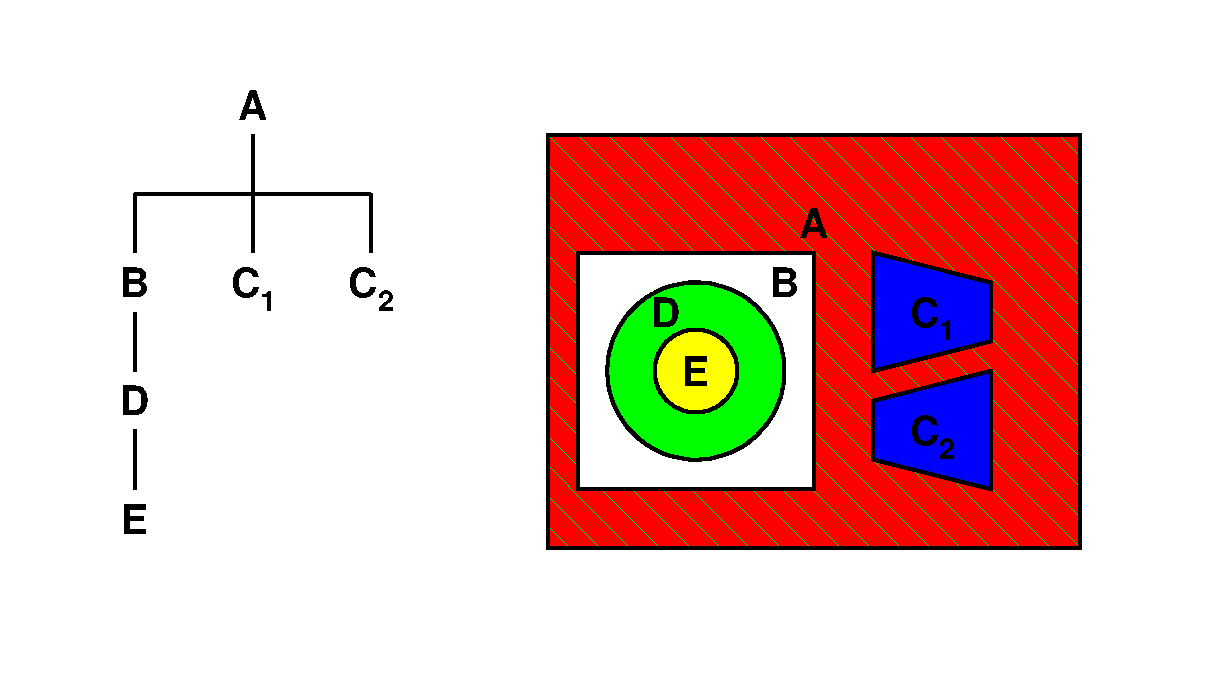
\epsfig{file=eps/geom001-1.eps,width=16cm}
      \caption{Example of geometrical tree structure}
      \label{fg:geom001-1}
\end{figure}

where A and B are {\tt BOX}es, C a {\tt TRAP}ezoid, and D and E {\tt TUBE}s
(see {\tt [GEOM050]} for more detail).
Notice that the same physical configuration could be described as well though
a 3 level tree if D were defined as a {\it hollow}
{\tt TUBE}, with inner radius non-zero and E
directly positioned into B.
The package accepts a maximum of 15 levels, which should be
enough to represent the fine details of a complex structure.
\section{The data structures {\tt JVOLUM} and {\tt JGPAR}
and the common {\tt /GCVOLU/}}

In practice, the physical tree is not represented as such in the
data part of the program. Instead, a logical tree structure is defined,
the {\tt JVOLUM} data structure, which describes the arrangement of
volumes in a compact and recurrent way. Each generic volume appears once,
and once only, and carries the information relevant to the volume itself
and to its contents, if any, by reference to the
generic volumes corresponding to those contents.
In the situation where division or multiple copies occur, there
is no longer a one-to-one correspondence between a volume in the
logical tree and a region in space. Information has to be added at
tracking time to identify which division cell or which copy was considered
at each depth level along the path through the physical tree. This
information is stored by the subroutine \Rind{GMEDIA}/\Rind{GTMEDI}, for the
current point of the current track, in the common \FCind{/GCVOLU/}. It includes
the current level number {\tt NLEVEL} and, for each level, starting from the
first mother volume, the identification of the corresponding volume, e.g.:
{\tt NAME}, {\tt NUMBER}, {\tt 'ONLY'/'MANY'} flag, translation and rotation
with respect to the master reference frame and so on. 
The number of shape parameters
and pointers to the vector describing the actual values of those
parameters, for each level, are stored in the data part and in the link
part, of the data structure {\tt JGPAR}, respectively.

\section{The user tools }

The geometry through which the particles are transported is defined by the
user via a set of calls to subroutines of the {\tt GEANT} package.

The user can define a volume through a call to the subroutine:
\begin{DLtt}{MMMMMMMM}
\item[\Rind{GSVOLU}] define ({\it instantiate}) a volume by giving a 
{\tt NAME} and the actual parameters to a shape; the position of the volume 
inside the bank {\tt JVOLUM} is returned. If any of the parameters which
express a length is negative, {\tt GEANT} will assign to this parameter
at tracking time
the maximum value allowed, without protruding out of the mother 
which contains the particle transported.

A shape can be instantiated
into a volume also without actual parameters. These will then be supplied
when positioning each copy of the volume via the \Rind{GSPOSP} routine (see
below). This allows to have many {\it similar} volumes with the same name
and shape, but different actual parameters in each copy.
\end{DLtt}

The user can position a volume through a call to either one of the following 
subroutines:

\begin{DLtt}{MMMMMMMM}
\item[\Rind{GSPOS}] position a copy of a volume inside its mother with respect 
to the mother's reference system. A a point in space, a rotation matrix
index, a copy number and the {\tt 'ONLY'/'MANY'} flag are supplied;
\item[\Rind{GSPOSP}] position a copy of a volume which has been instantiated
without actual parameters inside its mother with respect to the mother reference
system. The parameters of the copy being positioned are supplied as well.
The volumes will be identified by name and copy number as for multiple copies
of the same volume.
\end{DLtt}
The user can divide a volume through a call to either one of the following
subroutines:

\begin{DLtt}{MMMMMMM}
\item[\Rind{GSDVN}] divide a volume in a given {\it number} of cells completely
filling the mother. In this case the cell tracking medium
is assumed to be the same as for the mother. See also \Rind{GSDVN2}.
\item[\Rind{GSDVT}] divide a volume with slices of a given {\it step}.
The cell tracking medium can be different from the one of the mother.
See also \Rind{GSDVT2}.
\item[\Rind{GSDVX}] divide a volume starting from a given offset. In addition 
to {\tt STEP} and {\tt NDIV} (with at least one of them positive to be 
effectively useful), the origin of the first cell, the cell tracking medium 
and eventually the computed (maximum) number of divisions must be specified.
\end{DLtt}


\section{Geometrical information retrieval}

The parameters of a volume may depend on the physical tree which leads to
this volume. The dimensions of one of the slices of a cone divided along
{\tt Z} depends on which slice we consider. So a volume is completely
defined only if we specify the path in the tree. This is composed by the
name and copy number of the volumes containing the one we are interested
in, from the first mother.

Given this information, the routine \Rind{GLVOLU} is capable to fill the
common \FCind{/GCVOLU/}, and the structure {\tt JGPAR} with the actual
parameters of the instance chosen.

%%%%%%%%%%%%%%%%%%%%%%%%%%%%%%%%%%%%%%%%%%%%%%%%%%%%%%%%%%%%%%%%%%%
%                                                                 %
%  GEANT manual in LaTeX form                                     %
%                                                                 %
%  Michel Goossens (for translation into LaTeX)                   %
%  Version 1.00                                                   %
%  Last Mod. Jan 24 1991  1300   MG + IB                          %
%                                                                 %
%%%%%%%%%%%%%%%%%%%%%%%%%%%%%%%%%%%%%%%%%%%%%%%%%%%%%%%%%%%%%%%%%%%
\Documentation{S.Giani, S.Ravndal}
\Submitted{10.03.94}      \Revised{10.03.94}
\Version{Geant 3.21}\Routid{GEOM010}
\Makehead{Tracking inside volumes and optimisation}



The tracking of particles through the geometrical data structure is the key
functionality of {\tt GEANT}. 
At every particle's step, the program must find the
volume where the particle is ({\tt GTMEDI}) and the next boundary it will cross
({\tt GTNEXT}). This can take
about $60\%$ of the total simulation time (even for detectors described
in an optimized way); therefore, a new logic has been introduced to minimize
the time spent for the search in the geometrical tree. 

\section{ Virtual divisions}

Instead of a linear or
binary search (time spent proportional or logarithmic with the number of
volumes, respectively), a `direct access' technique has been developed to
make the time basically independent from the number of volumes. Every volume
containing other volumes is `virtually' divided in equal slices at 
initialization time via the call to {\tt GGCLOS}
(the best axis is computed automatically). 
For each slice,
a data structure is filled with a list of the volumes 
identifiers intersecting such
slice. 
Slices with identical lists are pointing to the same contents
and are collected. At 
tracking time it is immediate to find in which slice the particle is and only
its contents have to be checked. The same is true to find the next boundary to
be crossed: only if the intersection point with a content lies outside the 
current collection of slices, the next one will be checked. The algorithm
gives in average about a factor 2 in speed for the overall simulation in the
large detectors. It also minimizes the dependency of the performance
on the skill and experience of the programmer and allows a fast tracking even
in geometrical structures received from CAD systems.

\section{ Other optimisation tools}

The following facilities are kept for backward compatibility reasons.
If called by the user, these optimisation tools are called at 
initialisation time, but not used at tracking time. Instead, the
new optimisation using 'virtual divisions' is performed.
If the user wants to use the older optimisation tools, he can 
recompile {\tt GEANT} 3.21 using the {\tt PATCHY} flag {\tt +OLD}.
\begin{enumerate}
\item \Rind{GSORD}/\Rind{GGORD}

From the position of the contents inside a given volume, the
subroutine \Rind{GSORD} computes fictitious
boundaries along the specified coordinate, simulating
a division with irregular step size. A binary search technique is used
to identify within which pseudo-cell the current point is. The slow process
of computing whether the point is inside or outside the contents is therefore
limited to the few (if any) volumes overlapping with that
pseudo-cell, as sketched in fig~\ref{fg:geom001-2}.

\begin{figure}[hbt]
      \centering
      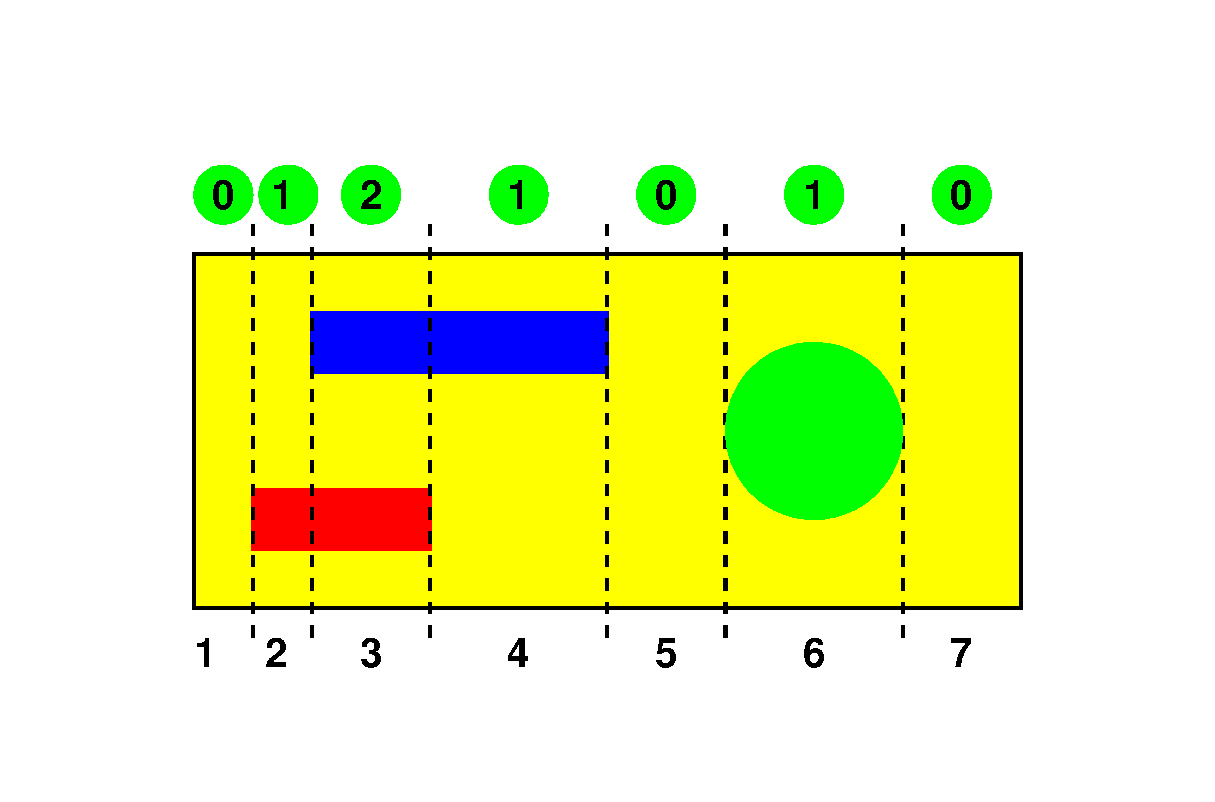
\epsfig{file=eps/geom001-2.eps,width=16cm}
      \caption{Example of pseudo-cells created by {\tt GSORD}}
      \label{fg:geom001-2}
\end{figure}

The coordinate selected for the pseudo division can be any of
{\tt X, Y, Z, $R_{xy}$, $R$, $\phi$ or $\theta$;}.
For a given volume, the call to \Rind{GSORD} has to come after all its first
level contents have been positioned.

\item
\Rind{GSNEXT}/\Rind{GSNEAR}

when a particle exits from a daugther of a 
mother volume, the contents are scanned initially
in the order in which 
they have been positioned, and the user should take care over
the best sequence of \Rind{GSPOS} calls. However, when the particle
{\it  comes back}
inside the mother from any one of the contents, it is
usually possible to limit the search to the neighbour contents.
The subroutines \Rind{GSNEXT}/\Rind{GSNEAR} permit the user to inject, at
initialisation time, for each content
in turn, the list of neighbours to search for.
\Rind{GSNEAR} is recommended, \Rind{GSNEXT} is kept for backward,
compatibility and has a different default option. A proper use of this
facility can reduce the search time significantly.

\item \Rind{GSUNEA}/\Rind{GUNEAR}

The volumes to be checked when exiting from one daughter can depend on 
the direction and position of the exiting particles. To optimise tracking
taking into account these dynamic features, the user can code the
\Rind{GUNEAR} routine, and inform {\tt GEANT} that it has to use it
at tracking time by calling the \Rind{GSUNEA} routine.
\end{enumerate}


%%%%%%%%%%%%%%%%%%%%%%%%%%%%%%%%%%%%%%%%%%%%%%%%%%%%%%%%%%%%%%%%%%%
%                                                                 %
%  GEANT manual in LaTeX form                                     %
%                                                                 %
%  Michel Goossens (for translation into LaTeX)                   %
%  Version 1.00                                                   %
%  Last Mod. Jan 24 1991  1300   MG + IB                          %
%                                                                 %
%%%%%%%%%%%%%%%%%%%%%%%%%%%%%%%%%%%%%%%%%%%%%%%%%%%%%%%%%%%%%%%%%%%
\Documentation{S.Giani, S.Ravndal}
\Submitted{22.03.94}      \Revised{22.03.94}
\Version{Geant 3.21}\Routid{GEOM020}
\Makehead{``MANY'' Volumes and boolean operations on volumes}

The topology of 
{\tt GEANT} is given by 16 general shapes which are used to represent
solids in the design of detectors. These shapes are bounded by 2-nd order
surfaces for reasons of speed at tracking time. New tools have been 
introduced to extend the power of the {\tt GEANT} geometry: boolean operations 
(union, intersection and subtraction) between such shapes are now allowed, so
that an infinity of new shapes can be built; divisions along arbitrary axis
are now possible, allowing to exploit any simmetry in the design.
The tracking is now able to handle overlapping volumes in the most general
sense: the concept of {\tt MANY} volumes has been extended to automatic 
clipping 
for protuding objects. Thanks to this {\tt MANY} technique, 
any 3D or 2D geometrical
pattern can be reduced to a single dimensional structure, basically cancelling
the need for {\tt GUNEAR} at tracking time. 
Finally, more than one order of magnitude in speed has been gained compared
to the old step search algorithm used to track in {\tt MANY} volumes. \\[.5cm]
\begin{itemize}
\item Topological extensions via boolean operations.
\item Divisions along arbitrary axis.
\item Reduction of 2D structure to 1D structure.
\item Logic and algorithm.
\end{itemize} 
 
\section{Topological extensions via boolean operations}

Boolean operations between a given set of shapes allow the creation of an
infinite number of shapes. Adding a single new primitive (for ex. a toroid) to 
the basic set of shapes, all the possible combinations with all the old shapes
become moreover possible.\\[.5cm]
\begin{itemize}
\item UNION: the union of two volumes B and C is obtained positioning two
             overlapping `{\tt MANY}' daughters B and C inside the same mother
             A.
             To identify the result of the union as a single volume is enough
             to create a SET associated to the volumes B and C. 
\item SUBTRACTION: the subtraction of a volume B from a volume C is obtained
                   positioning B as `{\tt ONLY}' and C as a `{\tt MANY}' 
                   overlapping B.
                   The result of the subtraction is automatically what the
                   tracking sees as the C volume, so {\tt GSPOS} is the only 
                   user
                   interface needed. The volume B can have the same material as
                   the mother A or not. The normal positioning technique used
                   for `{\tt ONLY}s' is a particular case of boolean subtraction (a
                   volume is contained inside the other).
\item INTERSECTION: the intersection of two volumes B and C is obtained 
                    positioning a protuding `{\tt MANY}' object C in 
                    a `{\tt MANY}' object
                    B which is normally placed in a `{\tt ONLY}' mother A. A and B
                    must have the same material, while C has the material asked
                    for the intersection. The intersection is given by the part
                    of C which is not protuding from B, therefore by what the
                    new tracking sees as the volume C: again the only needed
                    user interface is {\tt GSPOS}. If not interacting with other
                    daughters of A, B could also be `{\tt ONLY}'. Without any
                    ambiguity, even further `{\tt MANY}' daughters of A can overlap
                    the protuding part of C outside B, because it is really
                    invisible to the new tracking. 
\end{itemize}
 
\section{Divisions along arbitrary axis}

As protuding {\tt MANY} daughters are automatically clipped by their mother, 
it is
possible to divide objects along arbitrary directions. Suppose for example
that we want to divide a PCON into planar slices parallel to the plane
X + Y = 0; it is enough to position a {\tt MANY} BOX embedding completely the
PCON `inside' the PCON itself; the BOX must be rotated of 45 degrees in X and
Y and then divided along one of its natural axis. Another example can be the
following: suppose we want to divide 24 times in PHI a PGON with only 6 natural
segmentations in PHI; 
then we have to position a {\tt MANY} TUBE, completely embedding
the PGON, `inside' the PGON itself; again, we can now divide the tube in 24
slices in PHI and the tracking will see only the PGON divided 24 times in PHI.
\begin{center}
Reduction of 2D structure to 1D structure.
\end{center}
Sometimes there are complicated multidimensional geometrical structures (like
honeycombs, spaghetti, etc.) which can be reduced to the overlap of several
one-dimensional patterns (for which divisions can be used or virtual divisions
are particularly efficient). The {\tt MANY} option allows to superimpose such 1D
structures to reproduce the multi-dimensional ones in a very effective way,
instead of positioning the volumes one by one in the 2D or 3D pattern.
The following picture will explain better this concept.


\section{Logic and algorithm}

In {\tt GTMEDI}, all the '{\tt MANY}' volumes for which the point 
is found inside (and not
in any of its daughters) is put in a stack saving also its branch of the tree.
The point is considered to be in the deepest level 
'{\tt MANY}'. Each time the point
is also found in an intermediate '{\tt ONLY}' volume the stack is 
cleared (to insure
boolean subtraction). In {\tt GTNEXT}, if stepping 
inside a '{\tt MANY}' volume, not {\tt ONLY}
its daughters and its own boundaries are checked, but also the daughters and
the boundaries of all the others '{\tt MANY}' in the 
list have to be checked. This
is not yet enough: the logic requires that the boundaries of all the possible
overlapping volumes are checked, so it is also necessary for each `{\tt MANY}' 
volume 
of the list to go up to the first '{\tt ONLY}' mother 
in the tree repeating the same 
procedure. This allows also boolean intersection. Obviously, volumes already
checked are not checked again. 



%%%%%%%%%%%%%%%%%%%%%%%%%%%%%%%%%%%%%%%%%%%%%%%%%%%%%%%%%%%%%%%%%%%
%                                                                 %
%  GEANT manual in LaTeX form                              %
%                                                                 %
%  Michel Goossens (for translation into LaTeX)                   %
%  Version 1.00                                                   %
%  Last Mod. Jan 24 1991  1300   MG + IB                          %
%                                                                 %
%%%%%%%%%%%%%%%%%%%%%%%%%%%%%%%%%%%%%%%%%%%%%%%%%%%%%%%%%%%%%%%%%%%
\Origin{R.Brun, A.McPherson}
\Submitted{15.08.83}            \Revised{08.11.93}
\Version{Geant 3.16}\Routid{GEOM050}
\Makehead{The GEANT shapes}
 
The {\tt GEANT} geometry package offers sixteen basic shapes with which
to describe the setups where particles are transported. In this section
we will describe these shapes. For each shape figs~(\ref{fg:geom050-1}),
(\ref{fg:geom050-2}), (\ref{fg:geom050-3}), (\ref{fg:geom050-4}) 
show a simple drawing illustrating the
meaning of the parameters and the position and orientation of the
reference frame proper of that shape. A description of the shapes and of
their parameters follows. Angles are always in degrees. With every shape is
given the code which is used internally by {\tt GEANT} to identify it.
 
\begin{DLtt}{MMMMMMMM}
\item[1  BOX] box with faces perpendicular to the
axes. It has 3 parameters:
\begin{enumerate}
\item {\tt DX} half-length of the box along the x-axis;
\item {\tt DY} half-length of the box along the y-axis;
\item {\tt DZ} half-length of the box along the z-axis;
\end{enumerate}
 
\item[2  TRD1] trapezoid with the x dimension varying along z. It has
4 parameters:
\begin{enumerate}
\item {\tt DX1} half-length along x at the z surface positioned
at {\tt -DZ};
\item {\tt DX2} half-length along x at the z surface positioned
at {\tt +DZ};
\item {\tt DY} half-length along the y-axis;
\item {\tt DZ} half-length along the z-axis;
\end{enumerate}
 
\item[3  TRD2] trapezoid with both x and y dimensions varying along z.
It has 5 parameters:
\begin{enumerate}
\item {\tt DX1} half-length along x at the z surface positioned
at {\tt -DZ};
\item {\tt DX2} half-length along x at the z surface positioned
at {\tt +DZ};
\item {\tt DY1} half-length along y at the z surface positioned
at {\tt -DZ};
\item {\tt DY2} half-length along y at the z surface positioned
at {\tt +DZ};
\item {\tt DZ} half-length along the z-axis;
\end{enumerate}

\item[4  TRAP] {\it general} trapezoid: the
faces perpendicular to z are trapezia and their centres are not necessarily
on a line parallel to the z axis. This shape has 11 parameters, but only 
considering that the faces should be planar, only 9 are really independent.
A check is performed on the user parameters and a message is printed in
case of non-planar faces. Ignoring this warning may cause unpredictable
effect at tracking time.
\begin{enumerate}
\item {\tt DZ} half-length along the z axis;
\item {\tt THET} polar angle of the line joining the centre of the
face at {\tt -DZ} to the centre of the one at {\tt +DZ};
\item {\tt PHI} azimuthal angle of the line joining the centre of the
face at {\tt -DZ} to the centre of the one at {\tt +DZ};
\item {\tt H1} half-length along y of the face at {\tt -DZ};
\item {\tt BL1} half-length along x of the side at {\tt -H1}
in y of the face at {\tt -DZ} in z;
\item {\tt TL1} half-length along x of the side at {\tt +H1}
in y of the face at {\tt -DZ} in z;
\item {\tt ALP1} angle with respect to the y axis from the centre
of the side at {\tt -H1} in y to the centre 
of the side at {\tt +H1} in y of the face at {\tt -DZ} in z;
\item {\tt H2} half-length along y of the face at {\tt +DZ};
\item {\tt BL2} half-length along x of the side at {\tt -H2}
in y of the face at {\tt +DZ} in z;
\item {\tt TL2} half-length along x of the side at {\tt +H2}
in y of the face at {\tt +DZ} in z;
\item {\tt ALP2} angle with respect to the y axis from the centre
of the side at {\tt -H2} in y to the centre 
of the side at {\tt +H2} in y of the face at {\tt +DZ} in z;
\end{enumerate}
 
\item[5  TUBE] tube. It has 3 parameters:
\begin{enumerate}
\item {\tt RMIN} inside radius;
\item {\tt RMAX} outside radius;
\item {\tt DZ} half length in z;
\end{enumerate}

\item[6  TUBS] $\phi$ segment of a tube. It has 5 parameters:
\begin{enumerate}
\item {\tt RMIN} inside radius;
\item {\tt RMAX} outside radius;
\item {\tt DZ} half length in z;
\item {\tt PHI1} starting angle of the segment;
\item {\tt PHI2} ending angle of the segment;
\end{enumerate}
{\tt PHI1} should be smaller than {\tt PHI2}. If this is not the case,
the system adds 360 degrees to {\tt PHI2}.
 
\item[7  CONE] conical tube. It has 5 parameters:
\begin{enumerate}
\item {\tt DZ} half-length in z;
\item {\tt RMN1} inside radius at {\tt -DZ} in z;
\item {\tt RMX1} outside radius at {\tt -DZ} in z;
\item {\tt RMN2} inside radius at {\tt +DZ} in z;
\item {\tt RMX2} outside radius at {\tt +DZ} in z;
\end{enumerate}

 
\item[8  CONS] $\phi$ segment of a conical tube. It has 7 parameters:
\begin{enumerate}
\item {\tt DZ} half-length in z;
\item {\tt RMN1} inside radius at {\tt -DZ} in z;
\item {\tt RMX1} outside radius at {\tt -DZ} in z;
\item {\tt RMN2} inside radius at {\tt +DZ} in z;
\item {\tt RMX2} outside radius at {\tt +DZ} in z;
\item {\tt PHI1} starting angle of the segment;
\item {\tt PHI2} ending angle of the segment;
\end{enumerate}
{\tt PHI1} should be smaller than {\tt PHI2}. If this is not the case,
the system adds 360 degrees to {\tt PHI2}.

\item[9  SPHE] segment of spherical shell. It has 6 parameters:
\begin{enumerate}
\item {\tt RMIN} inside radius of the shell;
\item {\tt RMAX} outside radius of the shell;
\item {\tt THE1} starting polar angle of the shell;
\item {\tt THE2} ending polar angle of the shell;
\item {\tt PHI1} starting azimuthal angle of the shell;
\item {\tt PHI2} ending azimuthal angle of the shell;
\end{enumerate}
 
\item[10  PARA] parallelepiped. It has 6 parameters:
\begin{enumerate}
\item {\tt DX} half-length in x;
\item {\tt DY} half-length in y;
\item {\tt DZ} half-length in z;
\item {\tt ALPH} angle formed by the y axis and by the plane joining the
centre of the faces parallel to the z-x plane at {\tt -DY} and {\tt +DY};
\item {\tt THET} polar angle of the line joining the centres of the faces
at {\tt -DZ} and {\tt +DZ} in z;
\item {\tt PHI} azimuthal angle of the line joining the centres of the faces
at {\tt -DZ} and {\tt +DZ} in z;
\end{enumerate}

\item[11  PGON] {\it polygon}. It has at least 10 parameters:
\begin{enumerate}
\item {\tt PHI1} the azimuthal angle $\phi$ at which the volume {\it begins}
(angles are counted counterclockwise);
\item {\tt DPHI} {\it opening} angle of the volume, which extends from
{\tt PHI1} to {\tt PHI1+DPHI};
\item {\tt NPDV} number of sides of the cross section between the
given $\phi$ limits;
\item {\tt NZ} number of planes perpendicular to the z axis where the
dimension of the section is given -- this number should be at least
2 and {\tt NP} triplets of numbers must follow;
\item {\tt Z} z coordinate of the section;
\item {\tt RMIN} radius of the circle tangent to the sides of the inner
polygon in the cross-section;
\item {\tt RMAX} radius of the circle tangent to the sides of the outer
polygon in the cross-section;
\end{enumerate}

\item[12  PCON] {\it polycone}. It has at least 9 parameters:
\begin{enumerate}
\item {\tt PHI1} the azimuthal angle $\phi$ at which the volume {\it begins}
(angles are counted counterclockwise);
\item {\tt DPHI} {\it opening} angle of the volume, which extends from
{\tt PHI1} to {\tt PHI1+DPHI};
\item {\tt NZ} number of planes perpendicular to the z axis where the
dimension of the section is given -- this number should be at least
2 and {\tt NP} triplets of numbers must follow;
\item {\tt Z} z coordinate of the section;
\item {\tt RMIN} radius of the inner circle in the cross-section;
\item {\tt RMAX} radius of the outer circle in the cross-section;
\end{enumerate}

\item[13 ELTU] elliptical cross-section tube. It has three parameters:
\begin{enumerate}
\item {\tt P1} semi-axis of the ellipse along x;
\item {\tt P2} semi-axis of the ellipse along y;
\item {\tt DZ} half-length in z;
\end{enumerate}

The equation of the surface is $x^2\mbox{\tt P1}^{-2} + y^2
\mbox{\tt P2}^{-2} = 1$.

\item[14 HYPE] hyperbolic  tube, i.e. the inner and  outer surfaces are
hyperboloids, as would be formed by a system of cylindrical
wires  which were  then  rotated  tangentially about  their
centres. It has  4  parameters:
\begin{enumerate}
\item {\tt RMIN} inner radius at z=0, where tube is narrowest;
\item {\tt RMAX} outer radius at z=0, where tube is narrowest;
\item {\tt DZ} half-length in z;
\item {\tt THET} {\it stereo  angle} of rotation of the two faces;
\end{enumerate}

The hyperbolic  surfaces are  given by: $r^2 = (z \tan \theta )^2
+r_{z=0}^2$

\item[28  GTRA] general twisted trapezoid: the
faces perpendicular to z are trapezia and their centres are not necessarily
on a line parallel to the z axis as the {\tt TRAP}; additionally, the
faces may be {\it twisted} so that none of their edges are parallel. 
It is a {\tt TRAP} shape, except that it is {\it twisted}
in the x-y plane as a function of z. 
The parallel sides perpendicular to the z axis
are rotated with respect to the x axis by an angle {\tt
TWIST}, which is one of the parameters. The shape is defined by the eight
corners and is assumed to be constructed of straight lines joining points on
the boundary of the trapezoidal face at z=-DZ to the corresponding points on the
face at z=DZ. Divisions are not allowed.  It has 12 parameters: 
\begin{enumerate}
\item {\tt DZ} half-length along the z axis;
\item {\tt THET} polar angle of the line joining the centre of the
face at {\tt -DZ} to the centre of the one at {\tt +DZ};
\item {\tt PHI} azimuthal angle of the line joining the centre of the
face at {\tt -DZ} to the centre of the one at {\tt +DZ};
\item {\tt TWIST} {\it twist} angle of the faces parallel to the x-y plane
at z = $\pm${\tt DZ} around an axis parallel to z passing through their
centre;
\item {\tt H1} half-length along y of the face at {\tt -DZ};
\item {\tt BL1} half-length along x of the side at {\tt -H1}
in y of the face at {\tt -DZ} in z;
\item {\tt TL1} half-length along x of the side at {\tt +H1}
in y of the face at {\tt -DZ} in z;
\item {\tt ALP1} angle with respect to the y axis from the centre
of the side at {\tt -H1} in y to the centre 
of the side at {\tt +H1} in y of the face at {\tt -DZ} in z;
\item {\tt H2} half-length along y of the face at {\tt +DZ};
\item {\tt BL2} half-length along x of the side at {\tt -H2}
in y of the face at {\tt +DZ} in z;
\item {\tt TL2} half-length along x of the side at {\tt +H2}
in y of the face at {\tt +DZ} in z;
\item {\tt ALP2} angle with respect to the y axis from the centre
of the side at {\tt -H2} in y to the centre 
of the side at {\tt +H2} in y of the face at {\tt +DZ} in z;
\end{enumerate}

{\bf Note:} this shape suffers from the same limitations than the {\tt TRAP}:
the tracking routines assume that the faces are planar, but this constraint
is not easily expressed in terms of the 12 parameters. Additionally, no check
on the faces is performed in this case. Users should avoid to use this shape
as much as possible, and if they have to do so, they should make sure that the
faces are really planes. If this is not the case, the result of the transport
is unpredictable.

To accelerate the computations necessary for transport, 18 additional 
parameters are calculated for this shape:

\begin{enumerate}
\item {\tt DX0DZ} $dx/dz$ of the line joining the centres of the faces at 
z=$\pm${\tt DZ};
\item {\tt DY0DZ} $dy/dz$ of the line joining the centres of the faces at 
z=$\pm${\tt DZ};
\item {\tt X01} x at z=0 for line joining the
+ on parallel side, perpendicular corners at z=$\pm${\tt DZ};
\item {\tt Y01} y at z=0 for line joining the
+ on parallel side, + on perpendicular corners at z=$\pm${\tt DZ};
\item {\tt DXDZ1} $dx/dz$ for line joining the + on parallel side,
+ on perpendicular corners at z=$\pm${\tt DZ};
\item {\tt DYDZ1} $dy/dz$ for line joining the + on parallel side,
+ on perpendicular corners at z=$\pm${\tt DZ};
\item {\tt X02} x at z=0 for line joining the - on parallel side,
+ on perpendicular corners at z=$\pm${\tt DZ};
\item {\tt Y02} y at z=0 for line joining the - on parallel side,
+ on perpendicular corners at z=$\pm${\tt DZ};
\item {\tt DXDZ2} $dx/dz$ for line joining the - on parallel side,
+ on perpendicular corners at z=$\pm${\tt DZ};
\item {\tt DYDZ2} $dy/dz$ for line joining the - on parallel side, 
+ on perpendicular corners at z=$\pm${\tt DZ};
\item {\tt X03} x at z=0 for line joining the - on parallel side,
- on perpendicular corners at z=$\pm${\tt DZ};
\item {\tt Y03} y at z=0 for line joining the - on parallel side,
- on perpendicular corners at z=$\pm${\tt DZ};
\item {\tt DXDZ3} $dx/dz$ for line joining the - on parallel side,
- on perpendicular corners at z=$\pm${\tt DZ};
\item {\tt DYDZ3} $dy/dz$ for line joining the - on parallel side,
- on perpendicular corners at z=$\pm${\tt DZ};
\item {\tt X04} x at z=0 for line joining the + on parallel side,
- on perpendicular corners at z=$\pm${\tt DZ};
\item {\tt Y04} y at z=0 for line joining the + on parallel side,
- on perpendicular corners at z=$\pm${\tt DZ};
\item {\tt DXDZ4} $dx/dz$ for line joining the + on parallel side,
- on perpendicular corners at z=$\pm${\tt DZ};
\item {\tt DYDZ4} $dy/dz$ for line joining the + on parallel side,
- on perpendicular corners at z=$\pm${\tt DZ};
\end{enumerate}

\item[29 CTUB] {\it cut} tube, a tube cut at the extremities with planes
not necessarily perpendicular to the z axis. It has 11 parameters:
\begin{enumerate}
\item {\tt RMIN} inside radius;
\item {\tt RMAX} outside radius;
\item {\tt DZ} half length in z;
\item {\tt PHI1} starting angle of the segment;
\item {\tt PHI2} ending angle of the segment;
\item {\tt LX} x component of a unit vector perpendicular to the face at {\tt -DZ};
\item {\tt LY} y component of a unit vector perpendicular to the face at {\tt -DZ};
\item {\tt LZ} z component of a unit vector perpendicular to the face at {\tt -DZ};
\item {\tt HX} x component of a unit vector perpendicular to the face at {\tt +DZ};
\item {\tt HY} y component of a unit vector perpendicular to the face at {\tt +DZ};
\item {\tt HZ} z component of a unit vector perpendicular to the face at {\tt +DZ};
\end{enumerate}
{\tt PHI1} should be smaller than {\tt PHI2}. If this is not the case,
the system adds 360 degrees to {\tt PHI2}.
\end{DLtt}
\newpage
\begin{figure}[hbt]
\vspace{3cm}
      \centering
      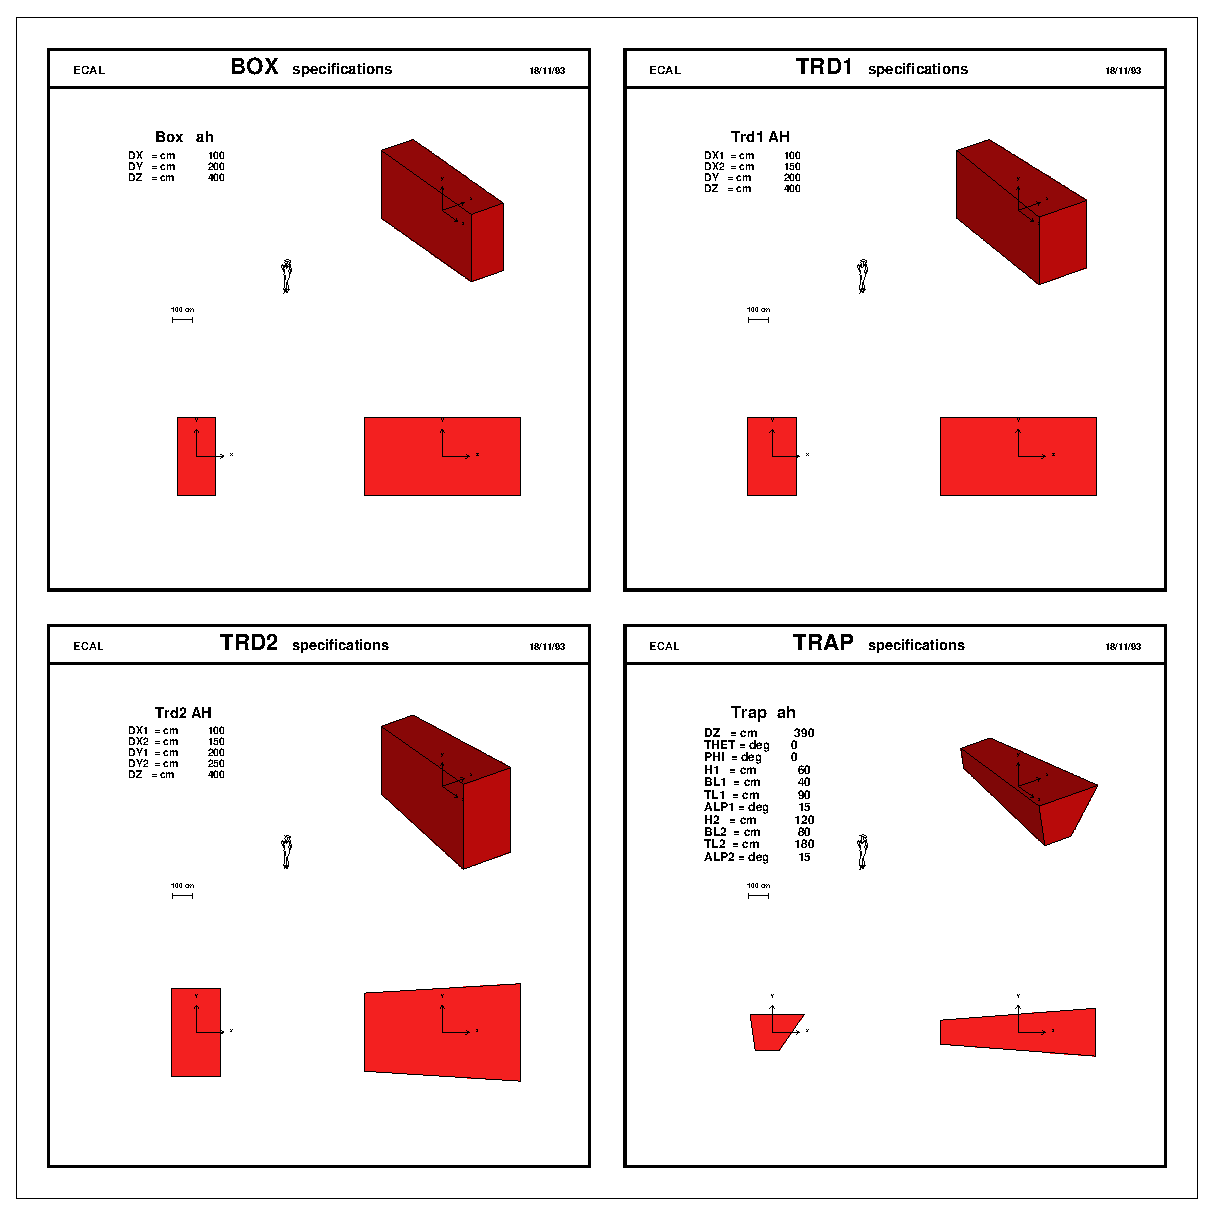
\epsfig{file=eps/geom050-1.eps,width=16cm}
      \caption{shapes {\tt BOX, TRD1, TRD2, TRAP}}
      \label{fg:geom050-1}
\end{figure}
\newpage
\begin{figure}[hbt]
\vspace{3cm}
      \centering
      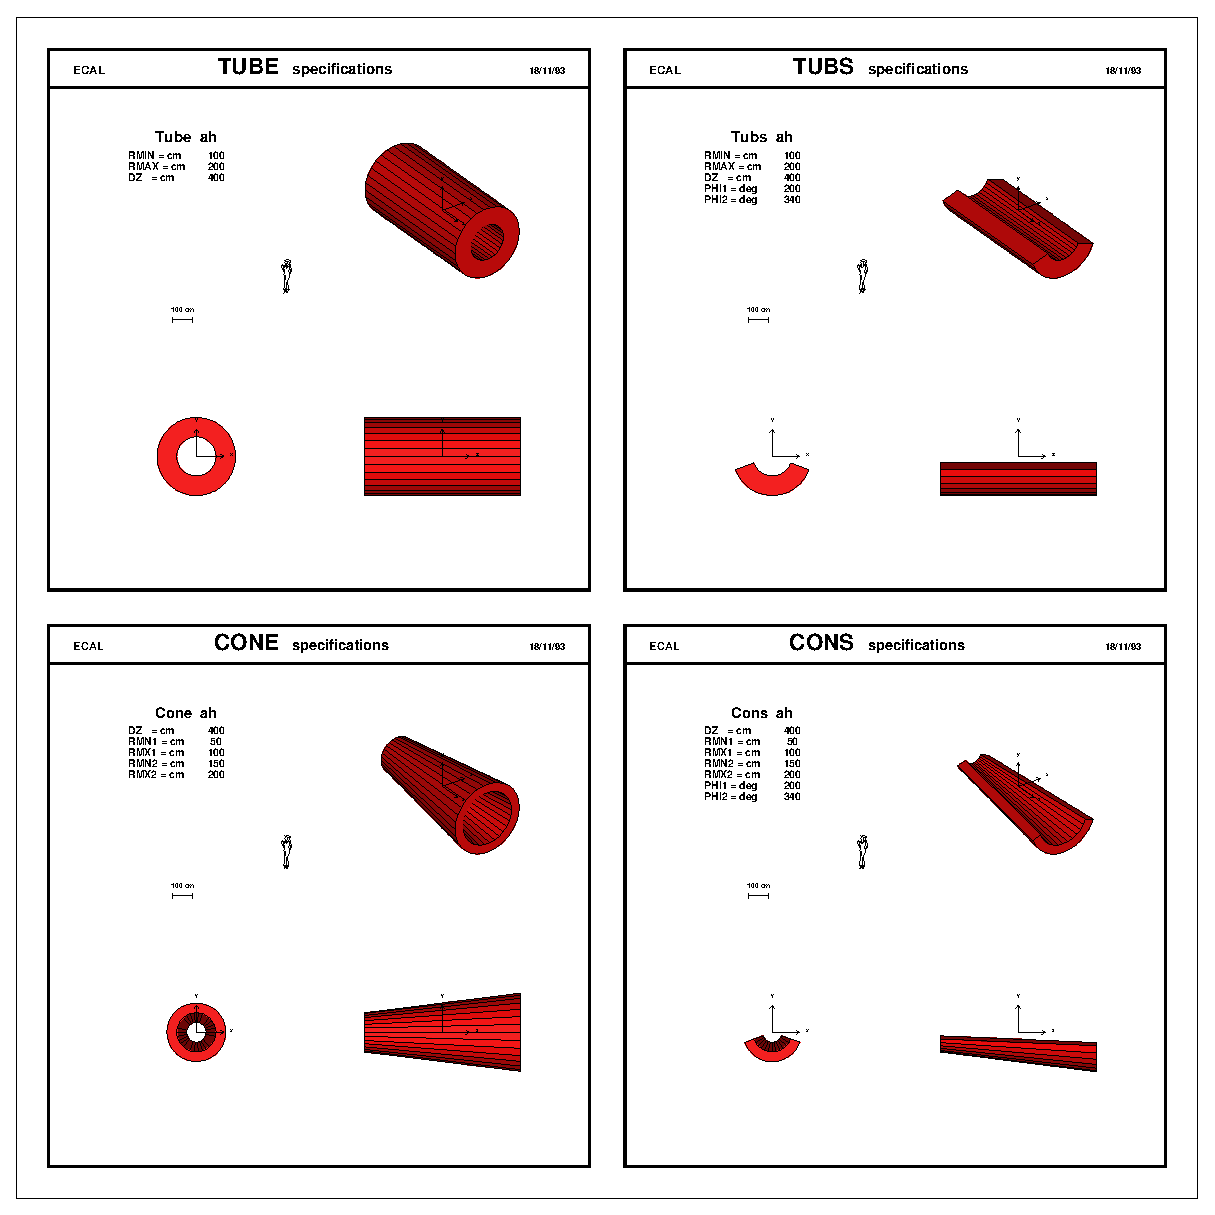
\epsfig{file=eps/geom050-2.eps,width=16cm}
      \caption{shapes {\tt TUBE, TUBS, CONE, CONS}}
      \label{fg:geom050-2}
\end{figure}
\newpage
\begin{figure}[hbt]
\vspace{3cm}
      \centering
      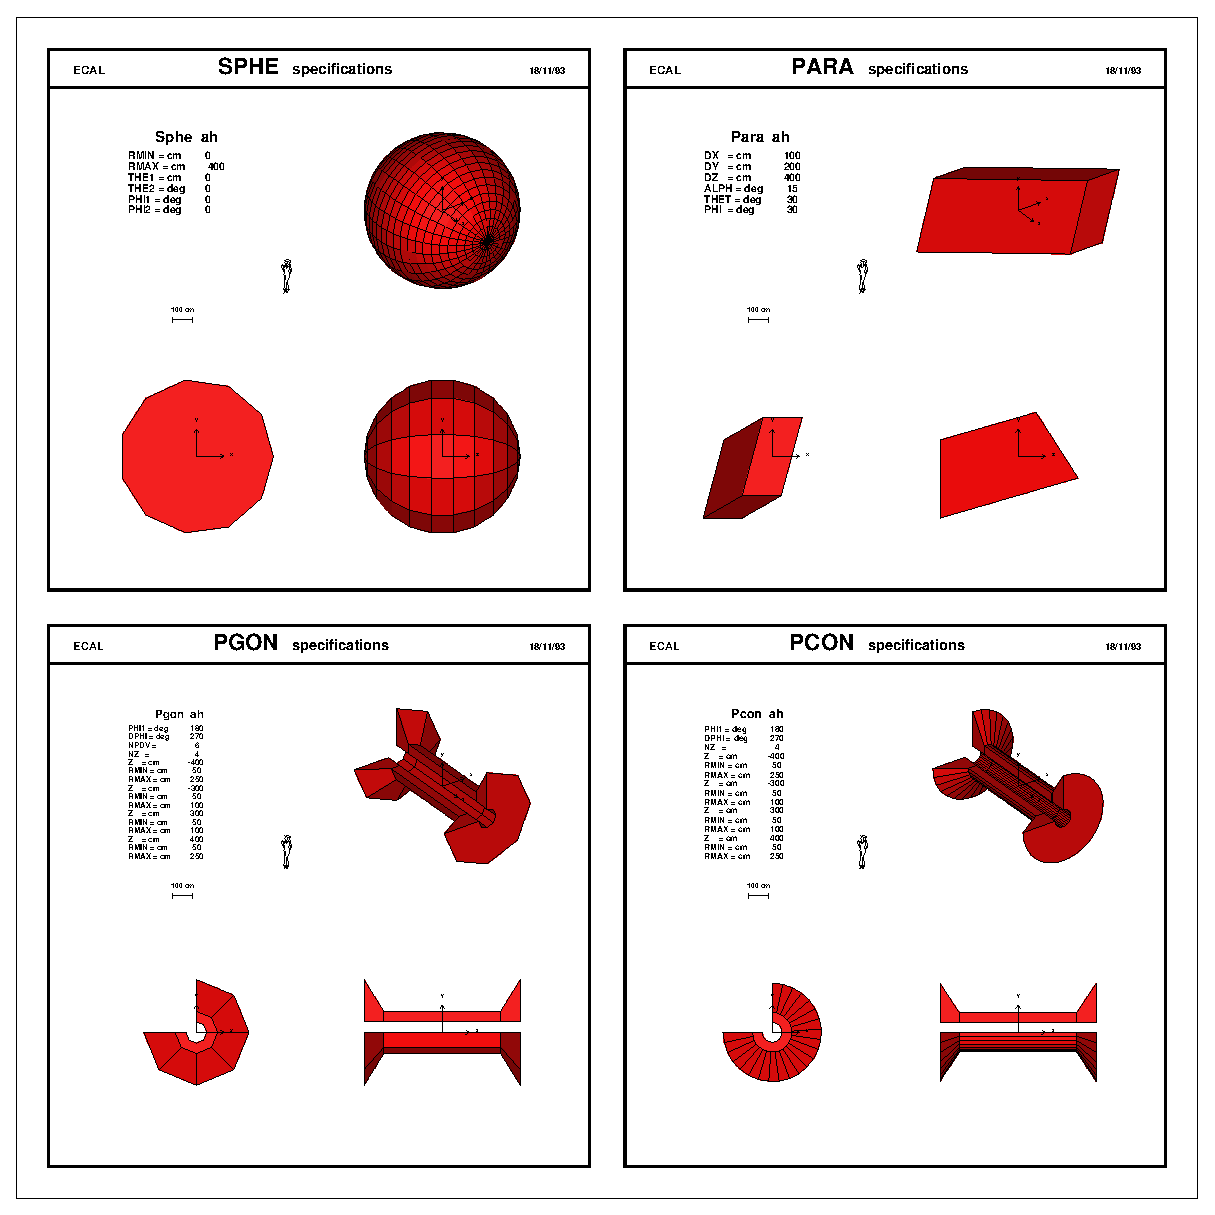
\epsfig{file=eps/geom050-3.eps,width=16cm}
      \caption{shapes {\tt PARA, SPHE, PGON, PCON}}
      \label{fg:geom050-3}
\end{figure}
\newpage
\begin{figure}[hbt]
\vspace{3cm}
      \centering
      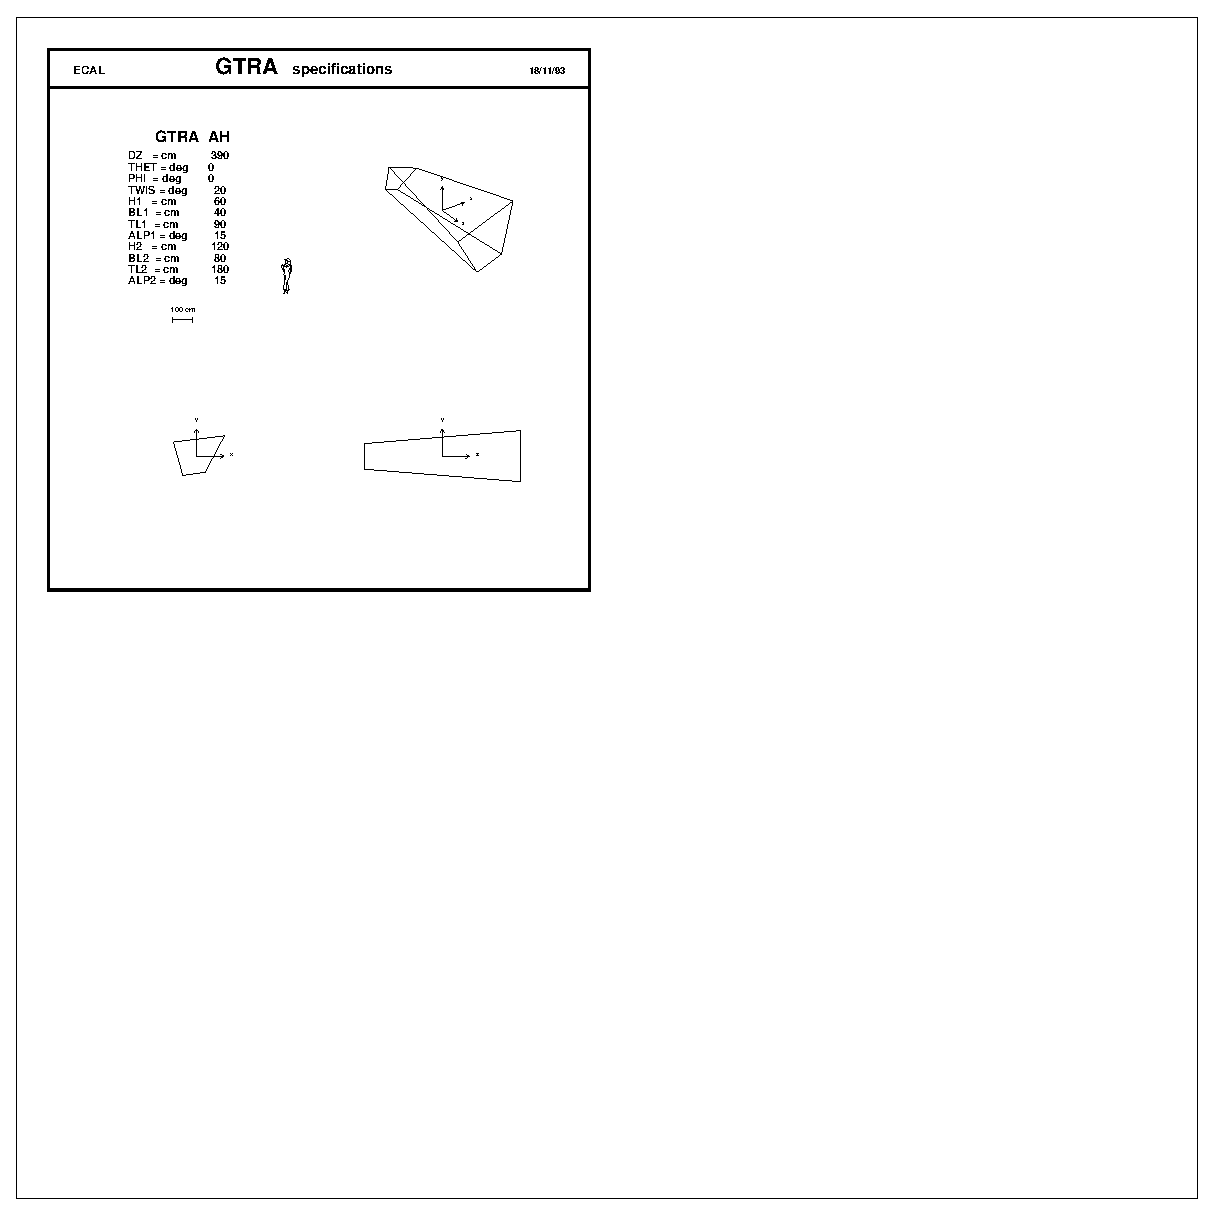
\epsfig{file=eps/geom050-4.eps,width=16cm}
      \caption{shapes {\tt GTRA}}
      \label{fg:geom050-4}
\end{figure}

%%%%%%%%%%%%%%%%%%%%%%%%%%%%%%%%%%%%%%%%%%%%%%%%%%%%%%%%%%%%%%%%%%%
%                                                                 %
%  GEANT manual in LaTeX form                              %
%                                                                 %
%  Michel Goossens (for translation into LaTeX)                   %
%  Version 1.00                                                   %
%  Last Mod. Jan 24 1991  1300   MG + IB                          %
%                                                                 %
%%%%%%%%%%%%%%%%%%%%%%%%%%%%%%%%%%%%%%%%%%%%%%%%%%%%%%%%%%%%%%%%%%%
\Origin{R.Brun,A.McPherson}
\Submitted{15.08.83}   \Revised{16.11.93}
\Version{Geant 3.16}   \Routid{GEOM100}
\Makehead{Creation of a volume}
 
\Shubr{GSVOLU}{(CHNAME,CHSHAP,NMED,PAR,NPAR,IVOLU*)}
Defines a volume with a given name, shape, tracking medium number
and shape parameters.

\begin{DLtt}{MMMMMMMM}
\item[CHNAME]  ({\tt CHARACTER*4}) volume name -- it must be unique;
\item[CHSHAP] ({\tt CHARACTER*4}) name of one of the {\tt GEANT} shapes;
\item[NMED]  ({\tt INTEGER}) tracking medium number for the volume --
if other volumes are positioned within this one, their tracking medium
replaces the one of the mother;
\item[PAR]   ({\tt REAL}) array containing the shape parameters;
\item[NPAR]  ({\tt INTEGER}) number of parameters -- if zero, then the
volume must be positioned via the routine \Rind{GSPOSP} indicating
the parameters for each copy (see {\tt [GEOM120]});
\item[IVOLU] ({\tt INTEGER}) internal volume number -- if $\leq 0$
an error condition has happened.
\end{DLtt}
 
If one of the parameters expressing a length is negative,
{\tt GEANT} will try to maximise its value in each copy, without
extending beyond the limits of the mother. This
facility can be used in conjunction with the
division of volumes using \Rind{GSDVN}, \Rind{GSDVT}, and \Rind{GSDVX}.
Restriction apply to this facility:
\begin{itemize}
\item the daughter should be positioned without a rotation matrix;
\item all shapes can be positioned within a similar shape with negative
parameters, but only in the centre of the mother;
\item boxes with negative parameters can be positioned in: box, {\tt TRD1},
{\tt TRD2} and {\tt TRAP} with $\theta = \phi = 0$;
\item {\tt HYPE}, {\tt ELTU} and {\tt CTUB} cannot have negative parameters;
\item {\tt PCON} and {\tt PGON} can only have 2 z planes.
\end{itemize}
{\bf Examples}
\begin{verbatim}
      DIMENSION PECAL(3)
      DATA PECAL/1.71,4.,0.2/
 
      CALL GSVOLU('ECAL','BOX ',1,PECAL,3,IVOLU)
\end{verbatim}
\Shubr{GPVOLU}{(IVOLU)}
Prints the volume parameters:
\begin{DLtt}{MMMM}
\item[IVOLU]  ({\tt INTEGER}) {\tt GEANT} number of the volume to print -- if
{\tt IVOLU} $\leq 0$, all volumes will be printed;
\end{DLtt}

%%%%%%%%%%%%%%%%%%%%%%%%%%%%%%%%%%%%%%%%%%%%%%%%%%%%%%%%%%%%%%%%%%%
%                                                                 %
%  GEANT manual in LaTeX form                                     %
%                                                                 %
%  Michel Goossens (for translation into LaTeX)                   %
%  Version 1.00                                                   %
%  Last Mod. Jan 24 1991  1300   MG + IB                          %
%                                                                 %
%%%%%%%%%%%%%%%%%%%%%%%%%%%%%%%%%%%%%%%%%%%%%%%%%%%%%%%%%%%%%%%%%%%
\Origin{R.Brun, A.McPherson}
\Submitted{15.08.83}              \Revised{16.11.93}
\Version{Geant 3.16}\Routid{GEOM110}

\Makehead{Positioning a volume inside its mother}

\Shubr{GSPOS}{(CHNAME,NR,CHMOTH,X,Y,Z,IROT,CHONLY)}
Places a copy of a volume previously defined by a call to \Rind{GSVOLU} 
inside its mother volume {\tt CHMOTH}.

\begin{DLtt}{MMMMMMMMMM}
\item[CHNAME] ({\tt CHARACTER*4}) name of the volume being positioned;
\item[NR] ({\tt INTEGER}) copy number of the volume {\tt CHNAME} being 
positioned;
\item[CHMOTH]({\tt CHARACTER*4}) name of the volume in which copy
{\tt NR} of {\tt CHNAME} is positioned;
\item[X] ({\tt REAL}) x position of the volume in the mother reference system;
\item[Y] ({\tt REAL}) y position of the volume in the mother reference system;
\item[Z] ({\tt REAL}) z position of the volume in the mother reference system;
\item[IROT] ({\tt INTEGER}) rotation matrix number
describing the orientation of the volume relative to
the coordinate system of the mother;
\item[CHONLY] ({\tt CHARACTER*4}) flag to indicate whether
a point found to be in this volume may also be in other volumes which
are not direct descendants of it -- possible values are {\tt ONLY} and
{\tt MANY}.
\end{DLtt}

The following points are important for a correct use of \Rind{GSPOS}:
\begin{itemize}
\item the position and rotation with which a volume is positioned are
relative to the mother reference system, that is to the reference system
of the volume which contains the copy being positioned. To see how the
reference system is defined for the {\tt GEANT} shapes, see {\tt [GEOM050]};
\item 
\Rind{GSPOS} can be called several times with the same name, to place 
multiple copies of the same volume either in the
same mother volume or in different ones.
The copy number parameter {\tt NR} is user defined, and it allows
the different copies of the same volume to be distinguished. The user is
free to assign any valid integer to this parameter. If two volumes
are positioned with the same copy number, it will be impossible to decide
in which one a particle is during tracking. If the same volume is positioned
twice inside the same mother with the same copy number, the parameters
of the second call to \Rind{GSPOS} will override the first ones for that
copy;
\item all the copies of a volume are identical: in particular they contain
all the same daughters recursively -- conversely, positioning a volume 
inside a mother will insert it in all the copies of that mother;
\item the volumes mentioned in the call must be already defined by a call
to \Rind{GSVOLU};
\item no volume can be positioned in a divided mother;
\item in case of positioning without rotation, {\tt IROT} should be set
to 0 -- note that this is faster than defining a unit matrix;
\item the first volume, containing all the apparatus, cannot be positioned;
\item if the {\tt CHONLY} flag is equal to {\tt ONLY}, the volume being
positioned should not overlap with any other volume except his mother
and his daughters and should not extend beyond the limits of its mother. 
In this case the search routines assume that, when a point
is found in this volume, the only further searching required is in its contents.
Other volumes at the same or higher levels
or in separate branches will not be looked at. The first volume must be 
{\tt ONLY};
\item if the {\tt CHONLY} flag is set to {\tt MANY}, a point found in
this volume can also be in another volume at the same or higher level or in
a different branch of the tree. To decide where a point is the following
algorithm is applied:
\begin{enumerate}
\item the tree is scanned {\it upward} until an {\tt ONLY} mother
with {\it positioned} contents (i.e. non-divided) is found;
\item all the branches of the tree descending from this volume are
scanned to find other volumes where the point may be;
\item a winner is selected among the candidates according to the
following rules:
\begin{itemize}
\item if one of the candidates is {\tt ONLY}, the point is declared in this
volume. If more than one candidate is {\tt ONLY} there is an error in the
geometry definition;
\item amongst several {\tt MANY} candidates, the one at the deepest level
is chosen;
\item amongst several {\tt MANY} candidates at the same level, the first one
found is chosen;
\end{itemize}
\end{enumerate}
Although a considerable effort has been put in making sure that the {\tt MANY}
option works properly and caters for all the possible cases, still it introduces
a considerable complication in the tracking and performance can be
rather poor.

Users should resort to this only when it is not possible to describe the
experimental setup with {\tt ONLY} volumes.
\end{itemize}

The data structure is so designed that, in any case, the parameters
of a volume and the information about the number and position of
its daughters are stored only once. This allows the creation of
very complex geometries without correspondingly large storage
requirements.

%%%%%%%%%%%%%%%%%%%%%%%%%%%%%%%%%%%%%%%%%%%%%%%%%%%%%%%%%%%%%%%%%%%
%                                                                 %
%  GEANT manual in LaTeX form                              %
%                                                                 %
%  Michel Goossens (for translation into LaTeX)                   %
%  Version 1.00                                                   %
%  Last Mod. Jan 24 1991  1300   MG + IB                          %
%                                                                 %
%%%%%%%%%%%%%%%%%%%%%%%%%%%%%%%%%%%%%%%%%%%%%%%%%%%%%%%%%%%%%%%%%%%
\Origin{R.Brun, F.Bruyant, M.Maire, A.McPherson}
\Submitted{15.08.83}               \Revised{18.11.93}
\Version{Geant 3.16}\Routid{GEOM120}
\Makehead{Positioning a volume inside its mother with parameters}

\Shubr{GSPOSP}{(CHNAME,NR,CHMOTH,X,Y,Z,IROT,CHONLY,PAR,NPAR)}

Position a copy of volume {\tt CHNAME} inside its mother {\tt CHMOTH}
assigning its parameters.

\begin{DLtt}{MMMMMMMMMM}
\item[CHNAME] ({\tt CHARACTER*4}) name of the volume being positioned;
\item[NR] ({\tt INTEGER}) copy number of the volume {\tt CHNAME} being
positioned;
\item[CHMOTH]({\tt CHARACTER*4}) name of the volume in which copy
{\tt NR} of {\tt CHNAME} is positioned;
\item[X] ({\tt REAL}) x position of the volume in the mother reference system;
\item[Y] ({\tt REAL}) y position of the volume in the mother reference system;
\item[Z] ({\tt REAL}) z position of the volume in the mother reference system;
\item[IROT] ({\tt INTEGER}) rotation matrix number
describing the orientation of the volume relative to
the coordinate system of the mother;
\item[CHONLY] ({\tt CHARACTER*4}) flag to indicate whether
a point found to be in this volume may also be in other volumes which
are not direct descendants of it -- possible values are {\tt ONLY} and
{\tt MANY};
\item[PAR] ({\tt REAL}) array of parameters for the volume being positioned;
\item[NPAR] ({\tt INTEGER}) number of parameters.
\end{DLtt}

It is often the case in a detector to have a family of similar objects,
differing only by their dimensions. A typical example are the crystals of
an electromagnetic calorimeter. In this case it is convenient and logically
consistent to give them all the same name, but assign to each copy a different
set of parameters.

This can be done defining the volume with 0 parameters through the routine
\Rind{GSVOLU} and then assigning the parameters to each copy via the routine
\Rind{GSPOSP}.

\Rind{GSPOSP} is similar in all other aspects to \Rind{GSPOS} and the user is
referred to the description of this routine for more information. An obvious
limitation is that a volume defined with 0 parameters can only be positioned
via \Rind{GSPOSP}, because otherwise its dimensions will be undefined.

%%%%%%%%%%%%%%%%%%%%%%%%%%%%%%%%%%%%%%%%%%%%%%%%%%%%%%%%%%%%%%%%%%%
%                                                                 %
%  GEANT manual in LaTeX form                                     %
%                                                                 %
%  Michel Goossens (for translation into LaTeX)                   %
%  Version 1.00                                                   %
%  Last Mod. Jan 24 1991  1300   MG + IB                          %
%                                                                 %
%%%%%%%%%%%%%%%%%%%%%%%%%%%%%%%%%%%%%%%%%%%%%%%%%%%%%%%%%%%%%%%%%%%
\Origin{R.Brun, A.McPherson}
\Submitted{29.09.83}             \Revised{18.11.93}
\Version{Geant 3.16}\Routid{GEOM130}
\Makehead{Division of a volume into a given number of cells}

\Shubr{GSDVN}{(CHNAME,CHMOTH,NDIV,IAXIS)}

Divide a volume in a given number of parts along a direction. 

\begin{DLtt}{MMMMMMMM}
\item[CHNAME] ({\tt CHARACTER*4}) a unique name for the volume to be generated
by subdivision of the mother volume;
\item[CHMOTH] ({\tt CHARACTER*4}) volume that has to be subdivided;
\item[NDIV] ({\tt INTEGER}) number of divisions into which the mother volume 
is to be divided;
\item[IAXIS] ({\tt INTEGER}) {\it axis} of the division.
\end{DLtt}

The volumes resulting from a division are true volumes in
the {\tt GEANT} sense, with the only limitation that they cannot be
positioned. They can have daughters and they can still be divided in turn.
Different divisions are distinguished by a different division number,
much the same as different copy of the same volume by the copy number.
Every operation performed on a division cell (positioning or further division),
is automatically propagated to all divisions cells of the same mother.

The kind of the division is indicated by the {\tt IAXIS} argument. 
The
allowed values of {\tt IAXIS} and the resulting divisions are shown in
figs. \ref{fg:geom130-1}, \ref{fg:geom130-2}, \ref{fg:geom130-3}, 
\ref{fg:geom130-4}, where the pictures in the first column correspond to 
an {\tt IAXIS} value equal to 1, the second column to {\tt IAXIS} = 2, 
and the third column to {\tt IAXIS} = 3 respectivly.
The
basic constraint imposed by the {\tt GEANT} geometry is that the result
of a division is a volume which can be described in terms of the basic 
shapes.

The local coordinate system of the divisions is parallel to the
system of the mother in case of divisions obtained by parallel planes or
concentric divisions. In the case of parallel axes the coordinate system
is shifted so that it is in the centre of the division.
In case of $\phi$ divisions produced by planes
passing through the axis of a volume with axial symmetry ({\tt TUBE, TUBS,
CONE, CONS, PGON, PCON, SPHE}), the local coordinate systems will be 
rotated so that the x axis passes through the centre of the division.

This routine allows the user to generate a large number of identical
volumes filling a defined volume. The material of the slices is inherited
from the mother.

It may happen that the different divisions of a volume have different
dimensions. In this case, if a volume has to be positioned in each division, 
its dimensions must be different according to the division number. This can
be obtained in some special cases giving to the dimension of the
volume which has to vary in order to fit into the different mothers,
the value of -1 in the call to
\Rind{GSVOLU} which defines it. As explained in {\tt [GEOM050]}, {\tt GEANT}
will take care to assign to this dimension the maximum value in order to
fill the current mother.

What can be done with division can be done also, in most cases, explicitly
positioning all the copies. Users must be aware, however, that divisions
offer the best performance in tracking of all {\tt GEANT} geometrical
constructs, and they should be used instead of positioning whenever
possible in the definition of objects.

\newpage
\begin{figure}[hbt]
      \centering
      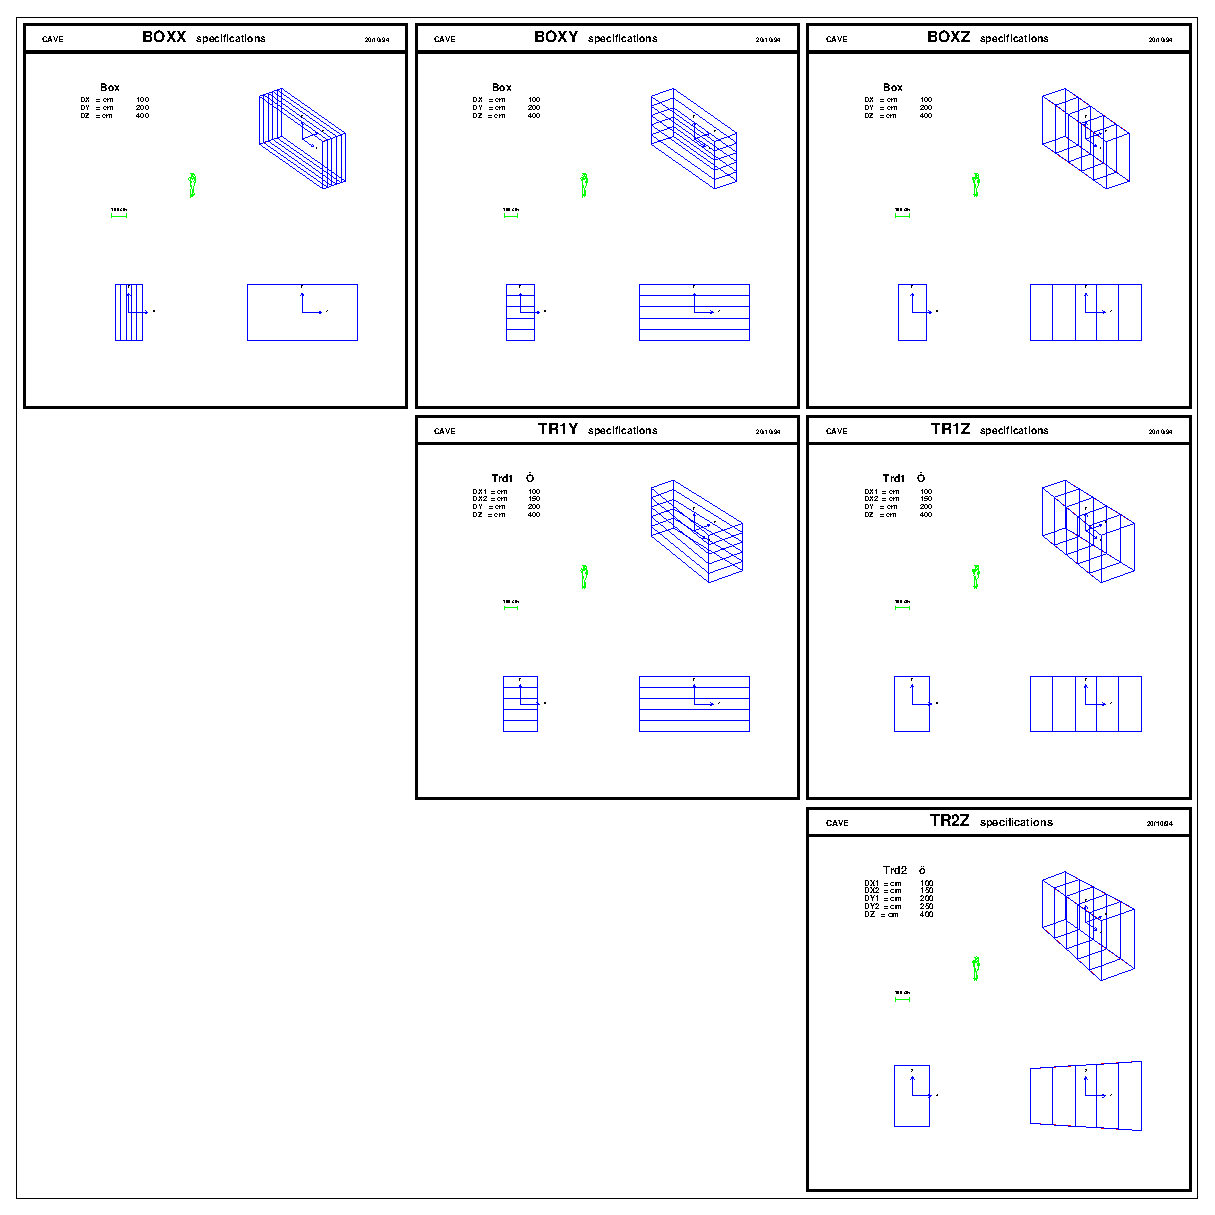
\epsfig{file=eps/geom130-1.eps,width=16cm}
      \caption{shapes {\tt BOX, TRD1, TRD2}}
      \label{fg:geom130-1}
\end{figure}
\newpage
\begin{figure}[hbt]
      \centering
      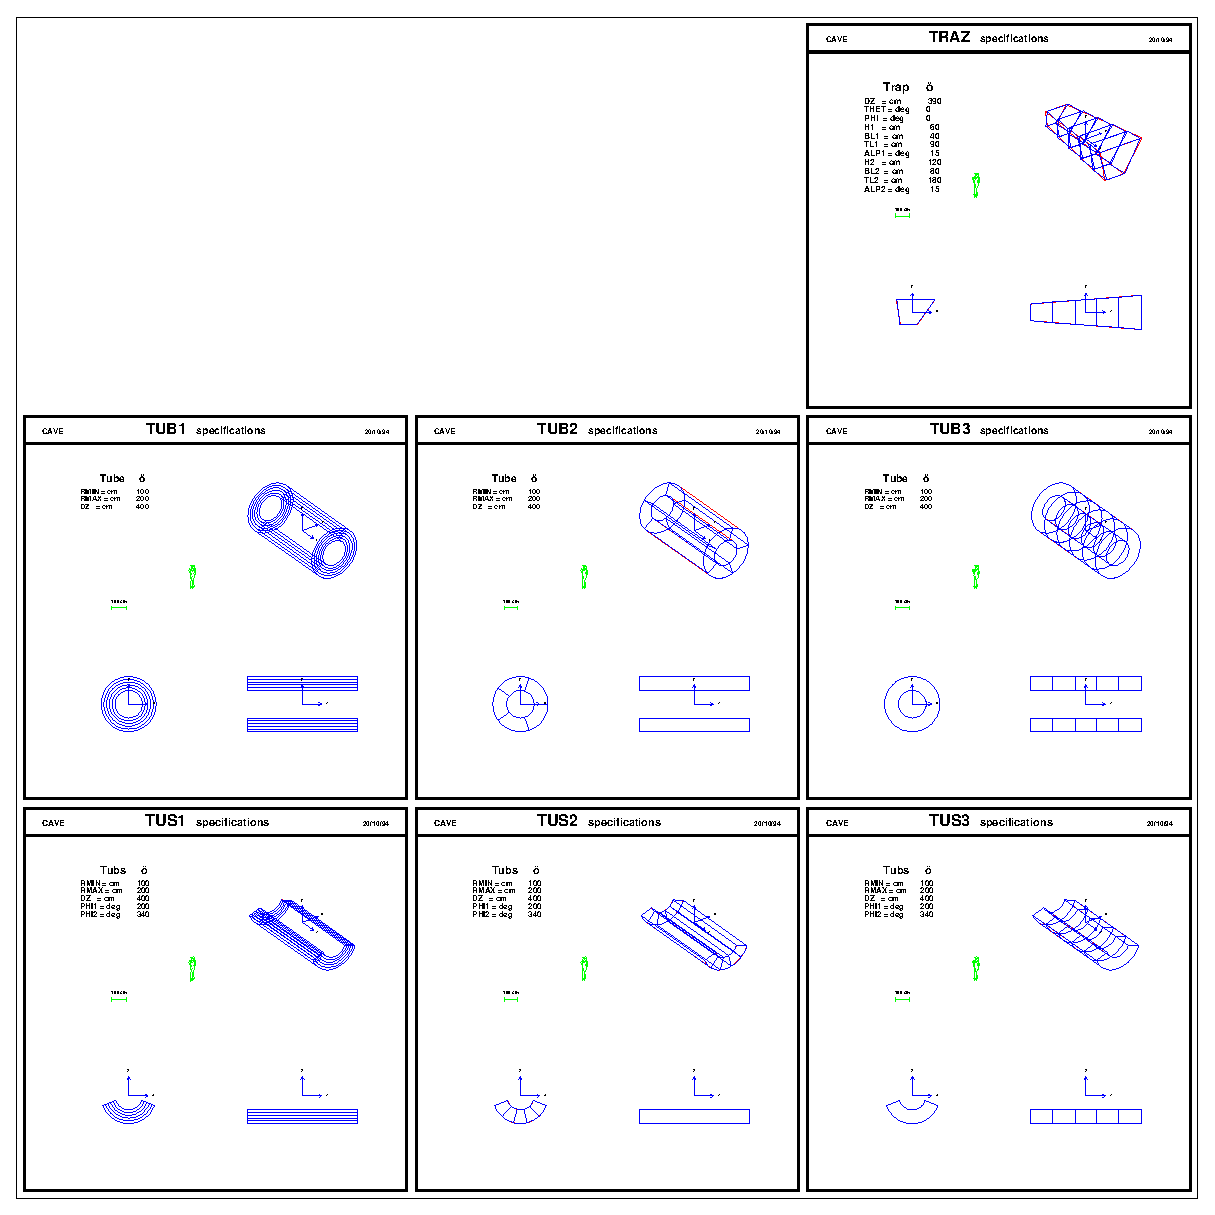
\epsfig{file=eps/geom130-2.eps,width=16cm}
      \caption{shapes {\tt TRAP, TUBE, TUBS}}
      \label{fg:geom130-2}
\end{figure}
\newpage
\begin{figure}[hbt]
      \centering
      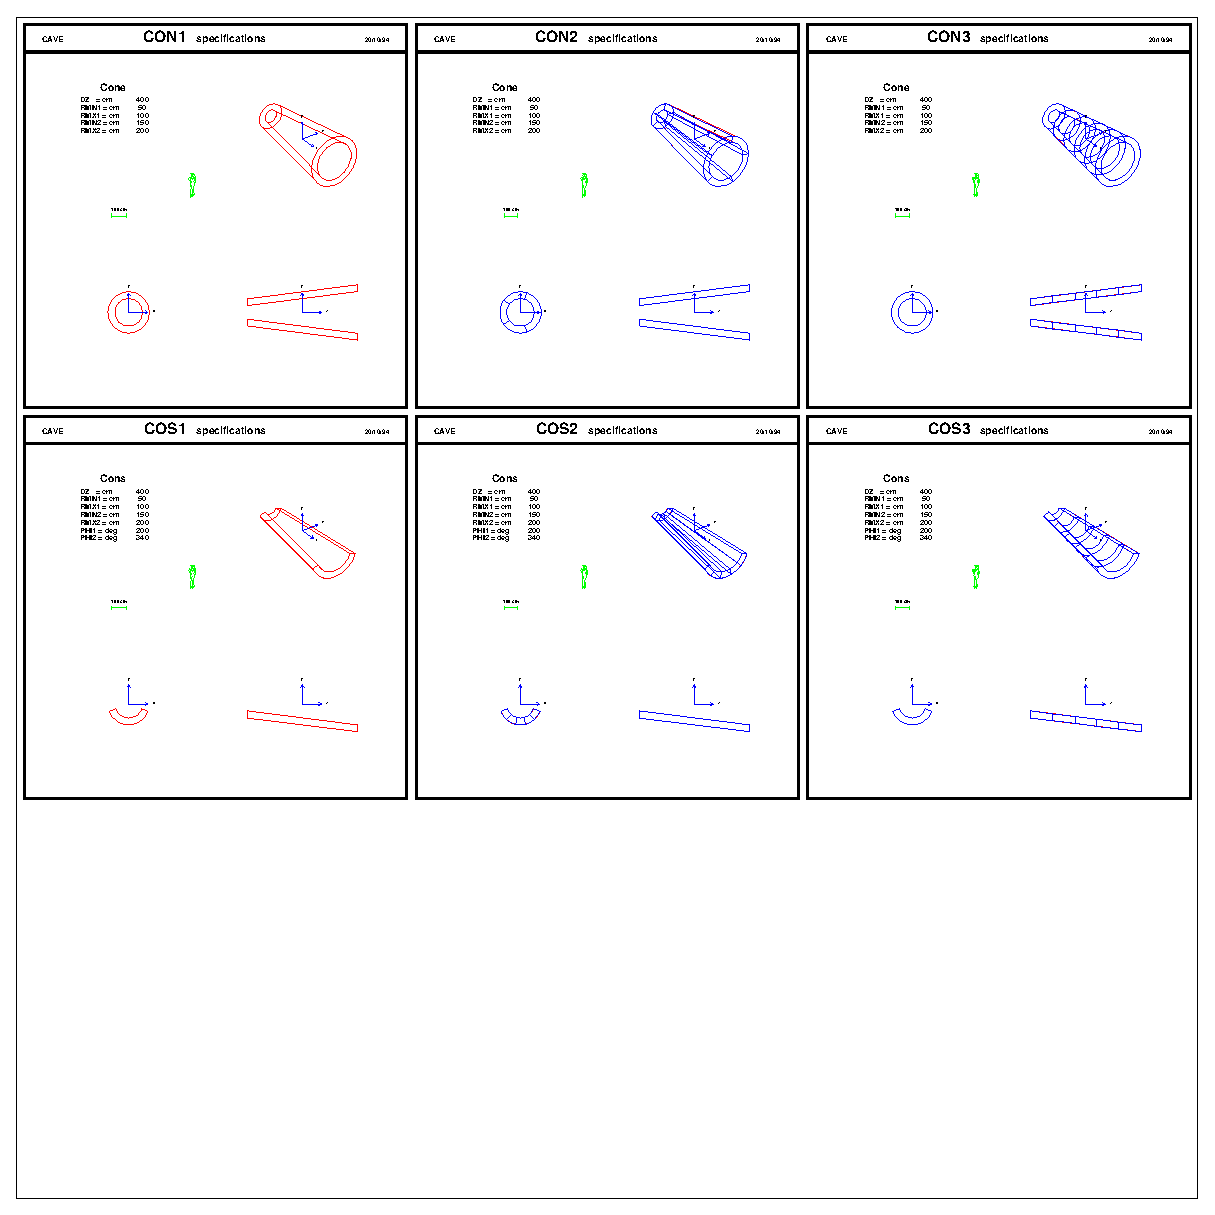
\epsfig{file=eps/geom130-3.eps,width=16cm}
      \caption{shapes {\tt CONE, CONS}}
      \label{fg:geom130-3}
\end{figure}
\newpage
\begin{figure}[hbt]
      \centering
      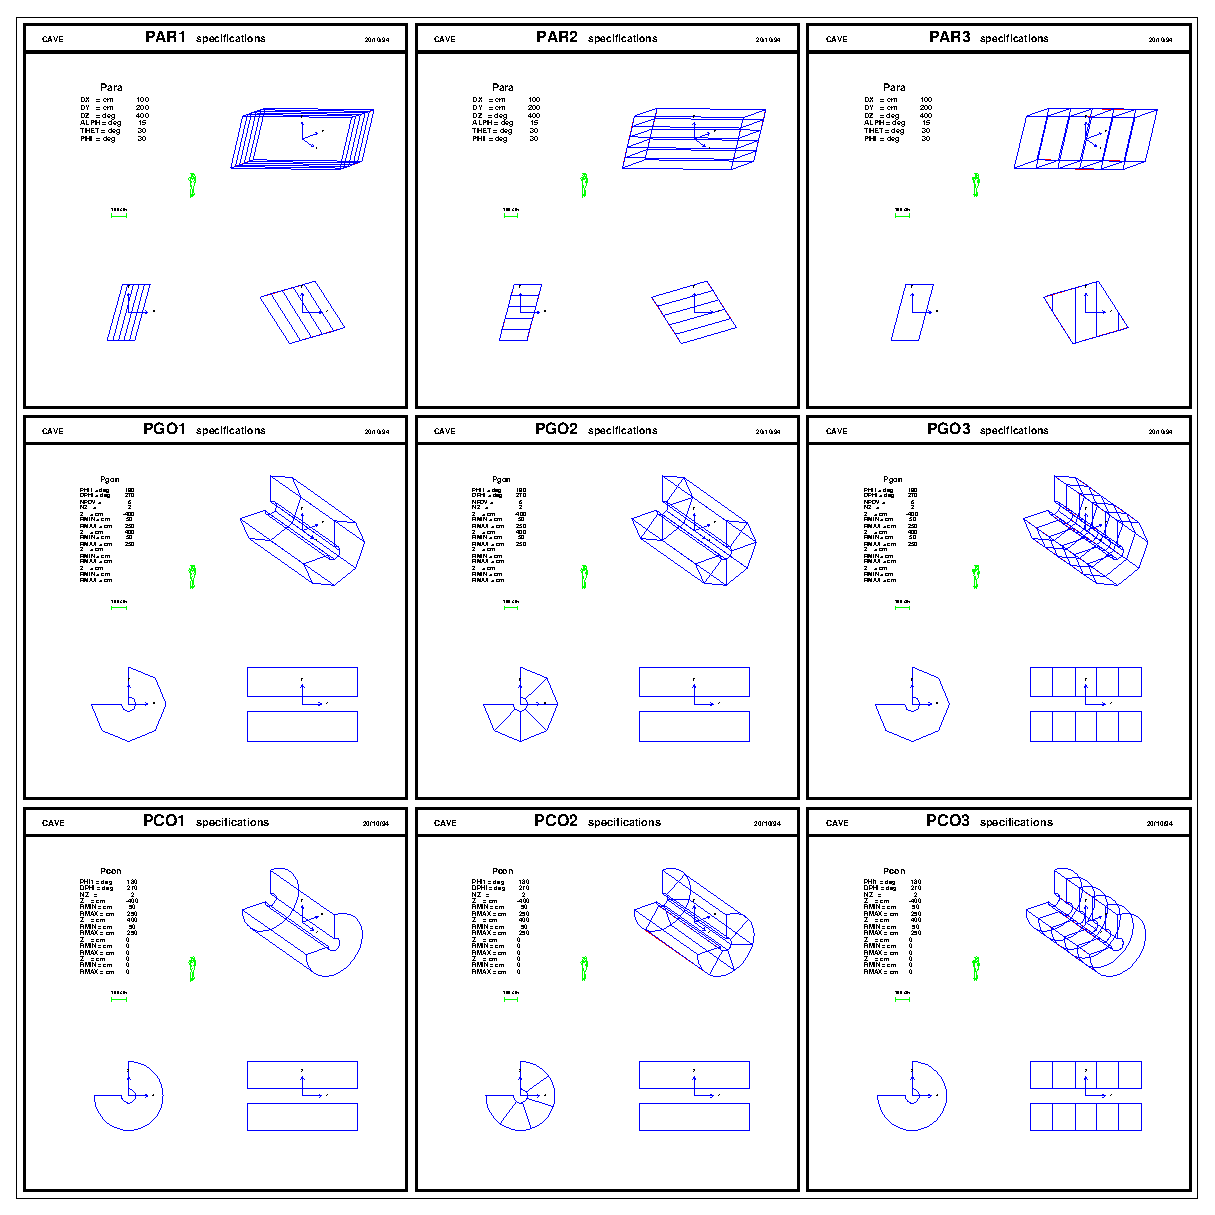
\epsfig{file=eps/geom130-4.eps,width=16cm}
      \caption{shapes {\tt PARA, PGON, PCON}}
      \label{fg:geom130-4}
\end{figure}

%%%%%%%%%%%%%%%%%%%%%%%%%%%%%%%%%%%%%%%%%%%%%%%%%%%%%%%%%%%%%%%%%%%
%                                                                 %
%  GEANT manual in LaTeX form                              %
%                                                                 %
%  Michel Goossens (for translation into LaTeX)                   %
%  Version 1.00                                                   %
%  Last Mod. Jan 24 1991  1300   MG + IB                          %
%                                                                 %
%%%%%%%%%%%%%%%%%%%%%%%%%%%%%%%%%%%%%%%%%%%%%%%%%%%%%%%%%%%%%%%%%%%
\Origin{F.Bruyant, A.McPherson, M.Maire}
\Submitted{17.12.83}       \Revised{18.11.93}
\Version{Geant 3.16}\Routid{GEOM140}
\Makehead{Division of a Volume into cells of a given size}

This routine creates new volumes from a mother 
by divisions of a given step.

\Shubr{GSDVT}{(CHNAME,CHMOTH,STEP,IAXIS,NUMED,NDVMX)}

\begin{DLtt}{MMMMMMMM}
\item[CHNAME] ({\tt CHARACTER*4}) a unique name for the volume to be generated
by subdivision of the mother volume;
\item[CHMOTH] ({\tt CHARACTER*4}) volume that has to be subdivided;
\item[STEP] ({\tt REAL}) size of the divisions -- this value can be in 
centimeters or degrees according to the value of {\tt IAXIS};
\item[IAXIS] ({\tt INTEGER}) {\it axis} of the division.
\item[NUMED] ({\tt INTEGER}) medium number of the divisions -- this can be 
different from the one of the mother, as the division cells may leave a
portion of the mother undivided (see below) --
if {\tt NUMED} $\leq 0$  the medium of the mother;
\item[NDVMX] ({\tt INTEGER}) expected (maximum) number of divisions -- if
$ \leq 0 $ or $ > 255 $, 255 is assumed.
\end{DLtt}

The full range of the mother will be divided
in sections of the user supplied step. If the step is such that the mother
cannot be divided exactly, the largest possible number
of divisions will be generated, the excess space will be equally
divided between each end of the range of the mother. These extra
spaces will be assumed to belong to the mother.

For more information on the division in general, see {\tt [GEOM130]}.

%%%%%%%%%%%%%%%%%%%%%%%%%%%%%%%%%%%%%%%%%%%%%%%%%%%%%%%%%%%%%%%%%%%
%                                                                 %
%  GEANT manual in LaTeX form                              %
%                                                                 %
%  Michel Goossens (for translation into LaTeX)                   %
%  Version 1.00                                                   %
%  Last Mod. Jan 24 1991  1300   MG + IB                          %
%                                                                 %
%%%%%%%%%%%%%%%%%%%%%%%%%%%%%%%%%%%%%%%%%%%%%%%%%%%%%%%%%%%%%%%%%%%
\Origin{R.Brun, F.Bruyant, A.McPherson}
\Submitted{17.12.83}               \Revised{18.11.93}
\Version{Geant 3.16}\Routid{GEOM150}
\Makehead{Division of a volume - general case}

\Shubr{GSDVX}{(CHNAME,CHMOTH,NDIV,IAXIS,STEP,C0,NUMED,NDVMAX)}

Divide a volume in a given number of parts along a direction, with
a given step starting from an offset.

\begin{DLtt}{MMMMMMMM}
\item[CHNAME] ({\tt CHARACTER*4}) a unique name for the volume to be generated
by subdivision of the mother volume;
\item[CHMOTH] ({\tt CHARACTER*4}) volume that has to be subdivided;
\item[NDIV] ({\tt INTEGER}) number of divisions into which the mother volume
is to be divided;
\item[IAXIS] ({\tt INTEGER}) {\it axis} of the division.
\item[STEP] ({\tt REAL}) size of the divisions -- this value can be in
centimeters or degrees according to the value of {\tt IAXIS};
\item[C0] ({\tt REAL}) offset where division should start -- this value can be 
in centimeters or degrees according to the value of {\tt IAXIS};
\item[NUMED] ({\tt INTEGER}) medium number of the divisions -- this can be
different from the one of the mother, as the division cells may leave a
portion of the mother undivided (see below) --
if {\tt NUMED} $\leq 0$  the medium of the mother;
\item[NDVMX] ({\tt INTEGER}) expected (maximum) number of divisions -- if
$ \leq 0 $ or $ > 255 $, 255 is assumed.
\end{DLtt}

For more information on the division mechanism, see {\tt [GEOM130]} and
{\tt [GEOM140]}. For the moment either
{\tt NDIV} or {\tt STEP} must be set negative or 0, so that they
will be computed from the {\tt CHMOTH}'s size.
The case with both {\tt NDIV} and {\tt STEP}
positive is not coded yet. It would permit leaving different
gaps at both ends of the
{\tt CHMOTH}.

Provisionally the code consists of a call to either \Rind{GSDVN2} or
\Rind{GSDVT2}.

\Shubr{GSDVN2}{(CHNAME,CHMOTH,NDIV,IAXIS,C0,NUMED)}

Divide a volume in a given number of parts along a direction, 
starting from an offset.

\begin{DLtt}{MMMMMMMM}
\item[CHNAME] ({\tt CHARACTER*4}) a unique name for the volume to be generated
by subdivision of the mother volume;
\item[CHMOTH] ({\tt CHARACTER*4}) volume that has to be subdivided;
\item[NDIV] ({\tt INTEGER}) number of divisions into which the mother volume
is to be divided;
\item[IAXIS] ({\tt INTEGER}) {\it axis} of the division.
\item[C0] ({\tt REAL}) offset where division should start -- this value can be 
in centimeters or degrees according to the value of {\tt IAXIS};
\item[NUMED] ({\tt INTEGER}) medium number of the divisions -- this can be
different from the one of the mother, as the division cells may leave a
portion of the mother undivided (see below) --
if {\tt NUMED} $\leq 0$  the medium of the mother;
\end{DLtt}

The divisions start at the user specified coordinate value
and extend to the end of the volume. The range from this offset to
the upper coordinate limit of the mother volume will be divided
into the supplied number of cells. 
In the case of 
$\phi$ division of a complete tube or cone, the whole 360 degrees
will be divided into the user-supplied number of slices no matter
what the origin is. Specifying an origin for the division, in this
case, just moves the
division boundaries. This can be useful to avoid a rotation.
In all other cases the search routines will
assume that a point is in the mother if the coordinate value is
less than the value of the supplied offset.

\Shubr{GSDVT2}{(CHNAME,CHMOTH,STEP,IAXIS,C0,NUMED,NDVMX)}

Divide a volume along a direction with a given step starting from an offset.

\begin{DLtt}{MMMMMMMM}
\item[CHNAME] ({\tt CHARACTER*4}) a unique name for the volume to be generated
by subdivision of the mother volume;
\item[CHMOTH] ({\tt CHARACTER*4}) volume that has to be subdivided;
\item[STEP] ({\tt REAL}) size of the divisions -- this value can be in
centimeters or degrees according to the value of {\tt IAXIS};
\item[IAXIS] ({\tt INTEGER}) {\it axis} of the division;
\item[C0] ({\tt REAL}) offset where division should start -- this value can be
in centimeters or degrees according to the value of {\tt IAXIS};
\item[NUMED] ({\tt INTEGER}) medium number of the divisions -- this can be
different from the one of the mother, as the division cells may leave a
portion of the mother undivided (see below) --
if {\tt NUMED} $\leq 0$  the medium of the mother;
\item[NDVMX] ({\tt INTEGER}) expected (maximum) number of divisions -- if
$ \leq 0 $ or $ > 255 $, 255 is assumed.
\end{DLtt}

The division start at the user-specified coordinate value
and extend to the end of the volume. The range from origin to
upper coordinate limit of the mother volume is divided
in sections of the user supplied step. If the step is such that
the range of the mother cannot be filled with cells, the largest
possible number of cells is created.
The excess space up to the end
of the mother volume will be assumed to belong to the mother.

In the case of 
$\phi$ division of a complete tube or cone, the whole 360 degrees
will be filled with slices, no matter
what the origin is. Specifying an origin for the division, in this
case, just moves the
division boundaries. This can be useful to avoid a rotation.

In all other cases the search routines will
assume a point is just in the mother if the coordinate value is
less than the value of the user supplied origin.

%%%%%%%%%%%%%%%%%%%%%%%%%%%%%%%%%%%%%%%%%%%%%%%%%%%%%%%%%%%%%%%%%%%
%                                                                 %
%  GEANT manual in LaTeX form                              %
%                                                                 %
%  Michel Goossens (for translation into LaTeX)                   %
%  Version 1.00                                                   %
%  Last Mod. Jan 24 1991  1300   MG + IB                          %
%                                                                 %
%%%%%%%%%%%%%%%%%%%%%%%%%%%%%%%%%%%%%%%%%%%%%%%%%%%%%%%%%%%%%%%%%%%
\Origin{R.Brun,F.Bruyant,A.McPherson}
\Submitted{01.11.83}                     \Revised{18.11.93}
\Version{Geant 3.16}\Routid{GEOM199}
\Makehead{The volume data structure -- JVOLUM}

\section{The data structure {\tt JVOLUM} and {\tt JGPAR}}

The meaning of the variables in the data structure {\tt JVOLUM} shown
in fig. \ref{fg:geom199-1}
is the following:

\begin{DLtt}{MMMMMMMM}
\item[ISEARC] search flag {\tt [GEOM400], [GEOM410]}:
\begin{DLtt}{MMMM}
\item[$=$0] volume positioning order or ordering by \Rind{GSNEXT}/\Rind{GSNEAR};
\item[$<$0] binary search as defined by \Rind{GSORD};
\item[$>$0] user ordering \Rind{GSUNEA}/\Rind{GUNEAR};
\end{DLtt}
\item[ISHAPE] system shape number (see {\tt [GEOM050]};
\item[NIN] number of volumes contained in the mother volume --
if negative the volume is divided;
\item[NMED] medium number for the volume;
\item[NPAR] number of shape parameters;
\item[NATT] number of attributes;
\item[PAR] array of shape parameters;
\item[IAT] array of attributes;
\item[IAXIS] direction of the division (see {\tt [GEOM130]});
\item[IVO] system volume number;
\item[NDIV] number of divisions ({\tt -NDVMX}, if computed dynamically,
see {\tt [GEOM140]});
\item[C0] coordinate value at which the division starts;
\item[STEP] coordinate step for the division;
\item[NR] user copy number;
\item[IROT] rotation matrix number defining the orientation of the volume
with respect to the mother reference system;
\item[X,Y,Z] position of the volume with respect to the mother reference
system;
\item[KONLY] {\tt ONLY/MANY} flag, see {\tt [GEOM110]} for more information;
\end{DLtt}
 
\begin{figure}[hbt]
     \centering
     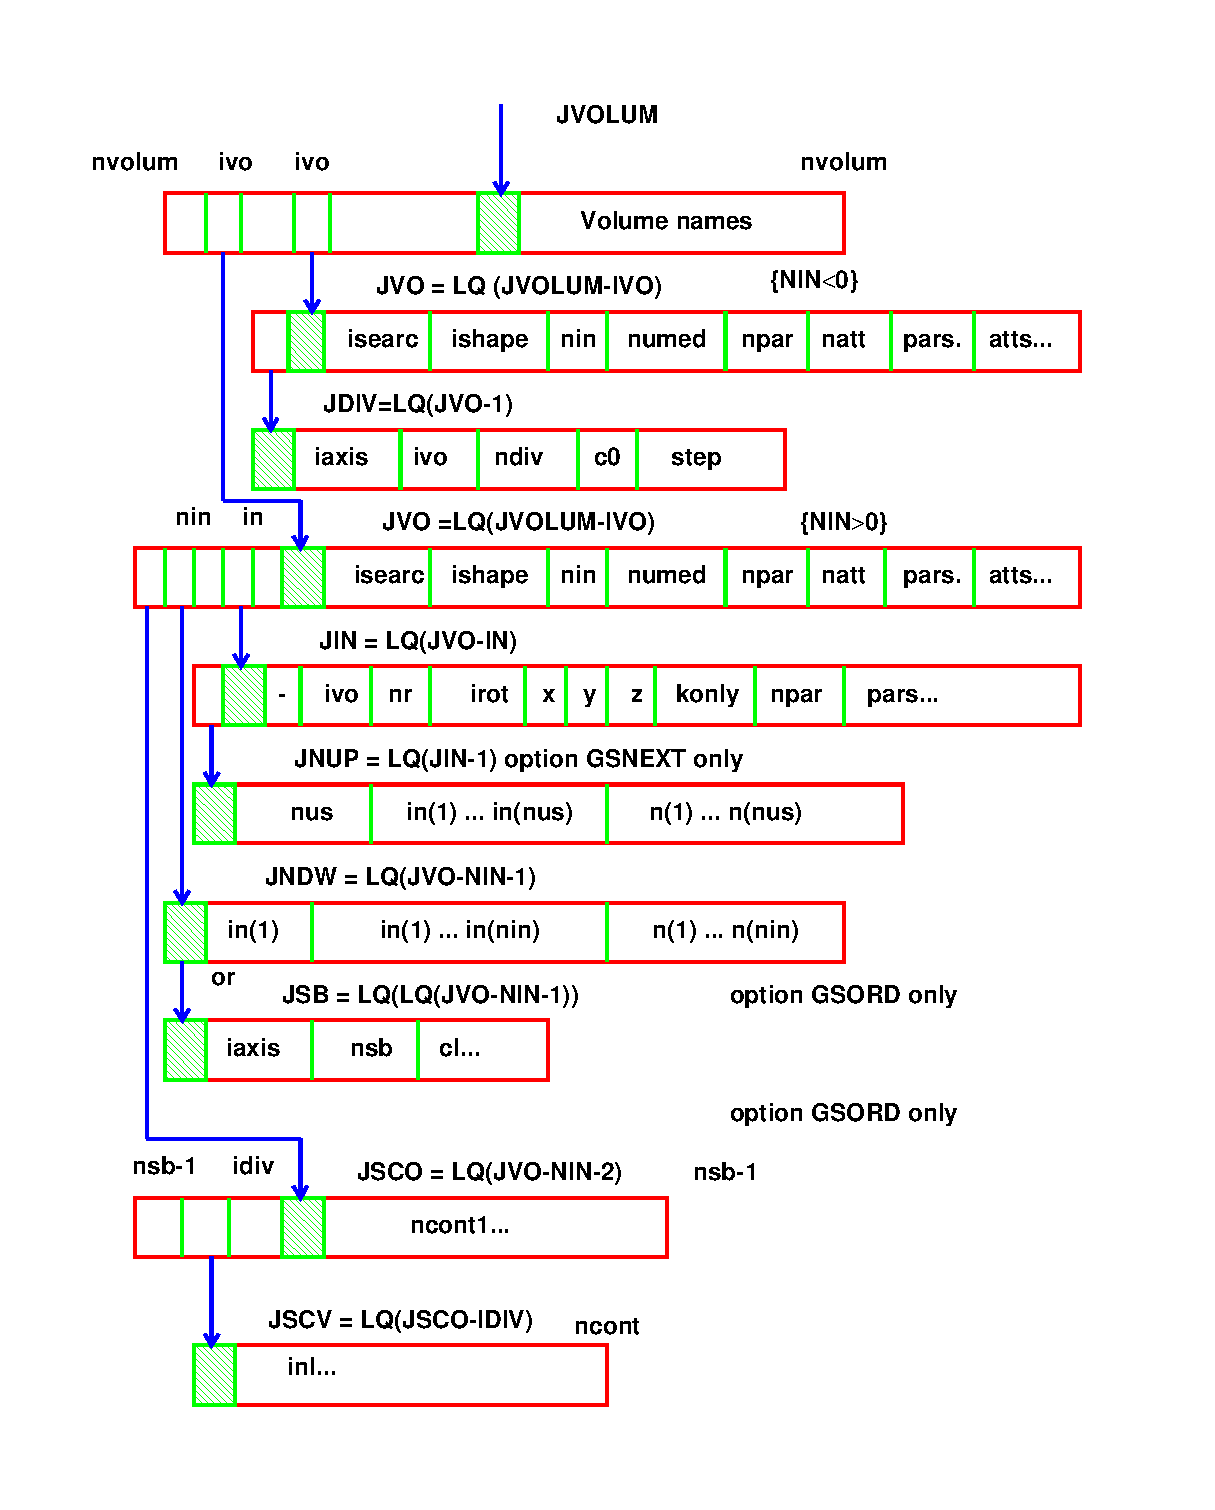
\epsfig{file=eps/geom199-1.eps,width=14cm}
     \caption{Example of geometrical tree structure}
     \label{fg:geom199-1}
\end{figure}

%%%%%%%%%%%%%%%%%%%%%%%%%%%%%%%%%%%%%%%%%%%%%%%%%%%%%%%%%%%%%%%%%%%
%                                                                 %
%  GEANT manual in LaTeX form                              %
%                                                                 %
%  Michel Goossens (for translation into LaTeX)                   %
%  Version 1.00                                                   %
%  Last Mod. Jan 24 1991  1300   MG + IB                          %
%                                                                 %
%%%%%%%%%%%%%%%%%%%%%%%%%%%%%%%%%%%%%%%%%%%%%%%%%%%%%%%%%%%%%%%%%%%
\Origin{R.Brun, F.Carena}
\Submitted{01.06.83}             \Revised{14.12.93}
\Version{Geant 3.16}\Routid{GEOM200}
\Makehead{Rotation matrices}

The relative position of a volume inside its mother is expressed in
{\tt GEANT} by a translation vector and a rotation matrix which are 
arguments of the routines \Rind{GSPOS} and \Rind{GSPOSP}. The rotation
matrix expresses the transformation from the {\tt M}other {\tt R}eference
{\tt S}ystem to the {\tt D}aughter {\tt R}eference {\tt S}ystem.

A rotation matrix is described to {\tt GEANT} by giving the polar and
azimuthal angles of the axes of the {\tt DRS} ($x', y', z'$) in the
{\tt MRS} via the routine \Rind{GSROTM}.

\Shubr{GSROTM}{(IROT,THETA1,PHI1,THETA2,PHI2,THETA3,PHI3)}
\begin{DLtt}{MMMMMMMM}
\item[IROT] ({\tt INTEGER}) number of the rotation matrix;
\item[THETA1] ({\tt REAL}) polar angle for axis $x'$;
\item[PHI1] ({\tt REAL}) azimuthal angle for axis $x'$;
\item[THETA2] ({\tt REAL}) polar angle for axis $y'$;
\item[THI2] ({\tt REAL}) azimuthal angle for axis $y'$;
\item[THETA3] ({\tt REAL}) polar angle for axis $z'$;
\item[PHI3] ({\tt REAL}) azimuthal angle for axis $z'$.
\end{DLtt}
Stores rotation matrix {\tt IROT} in the data structure {\tt JROTM}. If the
matrix is not orthonormal, it will be corrected by setting $y' \perp x'$ and
then $z' = x' \times y'$. A warning message is printed in this case.

{\bf Note:}
the angles {\tt THETA} and {\tt PHI} must be given in degrees.
 
\section*{Examples of use}
The unit matrix is defined in the following way:

\[
\left . \begin{array}{lcl}
x' & \| & x \\
y' & \| & y \\
z' & \| & z
\end{array} \right \}
\Rightarrow
\left \{
\begin{array}{lcr@{\mbox{\hspace{3mm};\hspace{8mm}}}lcr}
\theta_1 & = & 90^{\circ} & \phi_1 & = & 0^{\circ} \\
\theta_2 & = & 90^{\circ} & \phi_2 & = & 90^{\circ} \\
\theta_3 & = & 0^{\circ} & \phi_3 & = & 0^{\circ} 
\end{array} \right .
\]

This is just an example. There is in fact no need to define a unit rotation
matrix. Giving the value 0 to the rotation matrix number in the call to
\Rind{GSPOS} and \Rind{GSPOSP} is equivalent to a positioning without 
rotation and it improves tracking performance.

The result of a $90^{\circ}$ counterclockwise rotation around $z$, followed
by a $90^{\circ}$ counterclockwise rotation around the new $x$ is a cyclic
shift of the axes: $x \rightarrow z', \; y \rightarrow x', \; z \rightarrow  
y'$. This is expressed by the following rotation matrix:

\[
\left . \begin{array}{lcl}
x' & \| & y \\
y' & \| & z \\
z' & \| & x
\end{array} \right \}
\Rightarrow
\left \{
\begin{array}{lcr@{\mbox{\hspace{3mm};\hspace{8mm}}}lcr}
\theta_1 & = & 90^{\circ} & \phi_1 & = & 90^{\circ} \\
\theta_2 & = & 0^{\circ} & \phi_2 & = & 0^{\circ} \\
\theta_3 & = & 90^{\circ} & \phi_3 & = & 0^{\circ} 
\end{array} \right .
\]

Sometimes the rotation matrix is known or it can be constructed. In this case
the arguments to the routine \Rind{GSROTM} can be calculated with the help
of the routine \Rind{GFANG} in the following way:

\begin{verbatim}
      DIMENSION ROTMAT(3,3), ROWMAT(3), PHI(3), THETA(3)
      LOGICAL ROTATE
      .
      .
      .
      DO 10 I=1,3
         ROWMAT(1) = ROTMAT(I,1)
         ROWMAT(2) = ROTMAT(I,2)
         ROWMAT(3) = ROTMAT(I,3)
         CALL GFANG(ROWMAT,COSTH,SINTH,COSPH,SINPH,ROTATE)
         THETA(I) = ATAN2(SINTH,COSTH)
         PHI(I)   = ATAN2(SINPH,COSPH)
  10  CONTINUE
      .
      . {\sl Transform to degrees}
      .
      CALL GSROTM(IROT,THETA(1),PHI(1),THETA(2),PHI(2),THETA(3),PHI(3))
\end{verbatim}
 
\Shubr{GPROTM}{(IROT)}
Prints the rotation matrix elements and angles.
\begin{DLtt}{MMMMMMMM}
\item[IROT]  ({\tt INTEGER}) rotation matrix number: if {\tt IROT}=0 all
rotation matrixes will be printed, if {\tt IROT}$<$0, matrix number
{\tt |IROT|} will be printed without header information.
\end{DLtt}
 

%%%%%%%%%%%%%%%%%%%%%%%%%%%%%%%%%%%%%%%%%%%%%%%%%%%%%%%%%%%%%%%%%%%
%                                                                 %
%  GEANT manual in LaTeX form                              %
%                                                                 %
%  Michel Goossens (for translation into LaTeX)                   %
%  Version 1.00                                                   %
%  Last Mod. Jan 24 1991  1300   MG + IB                          %
%                                                                 %
%%%%%%%%%%%%%%%%%%%%%%%%%%%%%%%%%%%%%%%%%%%%%%%%%%%%%%%%%%%%%%%%%%%
\Origin{R.Brun}
\Submitted{01.11.78}     \Revised{14.12.93}
\Version{Geant 3.16}     \Routid{GEOM299}
\Makehead{The rotation matrix data structure JROTM}
 
\begin{figure}[hbt]
     \centering
     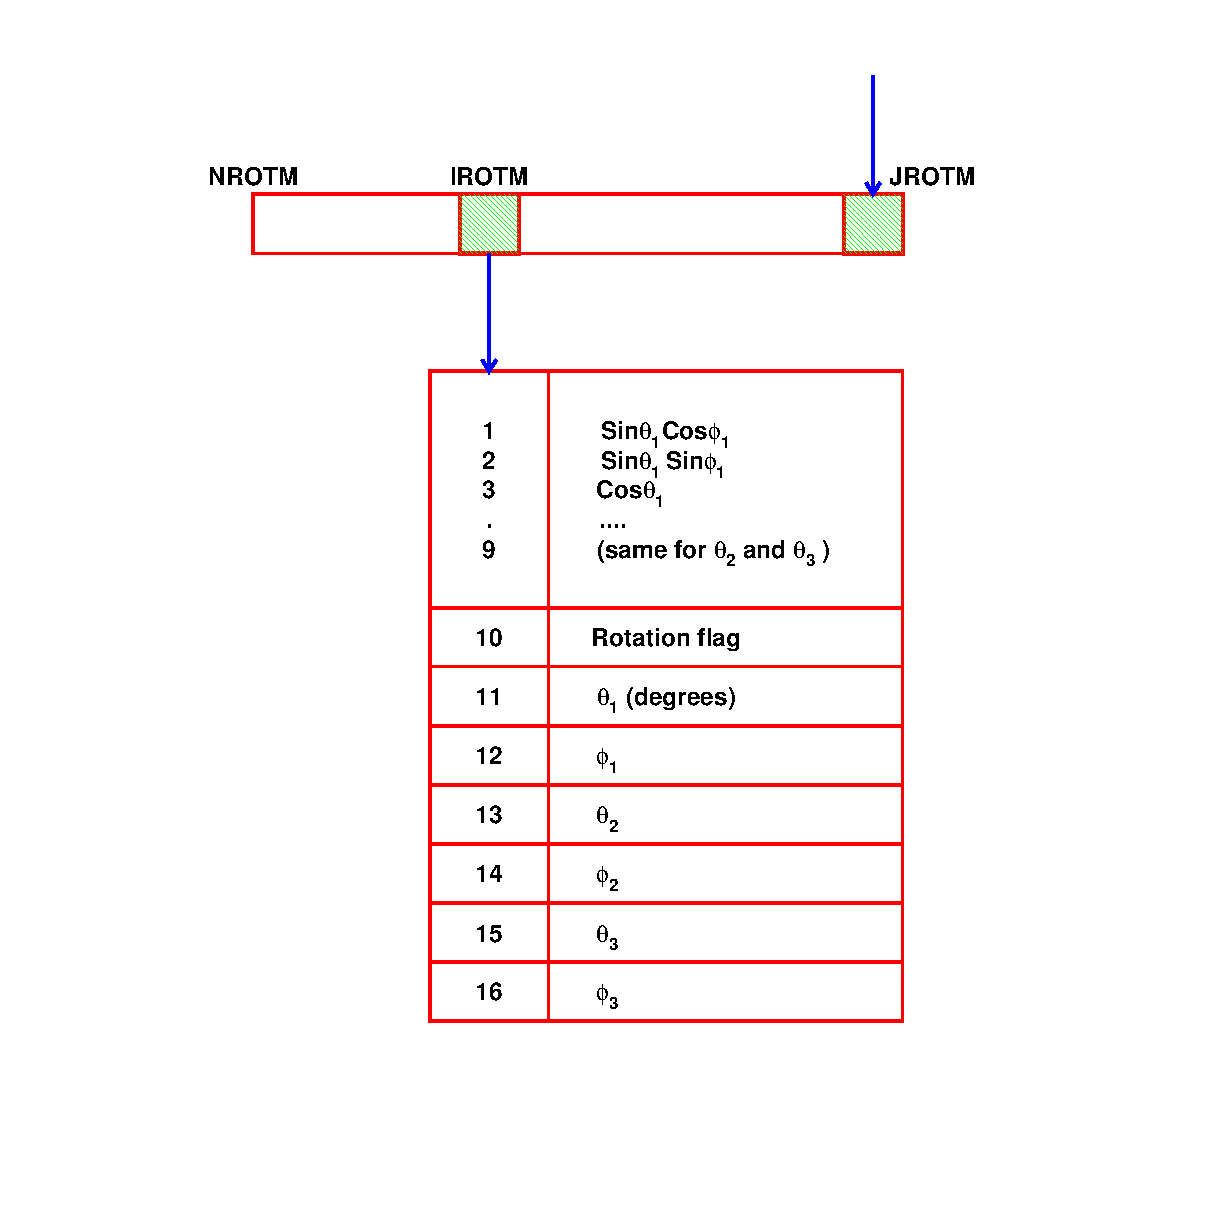
\epsfig{file=eps/geom299-1.eps,width=14cm}
     \caption{Layout of the {\tt JROTM} data structure}
     \label{fg:geom299-1}
\end{figure}

{\tt JR = LQ(JROTM-IROTM)} is the
pointer to the bank of the rotation matrix {\tt IROTM};
 
The rotation flag is computed by \Rind{GSROTM} to 
recognise simple rotation configurations. In particular it
is set to 0 for the unit matrix. 

%%%%%%%%%%%%%%%%%%%%%%%%%%%%%%%%%%%%%%%%%%%%%%%%%%%%%%%%%%%%%%%%%%%
%                                                                 %
%  GEANT manual in LaTeX form                              %
%                                                                 %
%  Michel Goossens (for translation into LaTeX)                   %
%  Version 1.00                                                   %
%  Last Mod. Jan 24 1991  1300   MG + IB                          %
%                                                                 %
%%%%%%%%%%%%%%%%%%%%%%%%%%%%%%%%%%%%%%%%%%%%%%%%%%%%%%%%%%%%%%%%%%%
\Origin{R.Brun, A.C.McPherson, F.Bruyant}
\Revision{S.Giani}
\Submitted{18.12.83}       \Revised{14.12.93}
\Version{Geant 3.16}       \Routid{GEOM300}

\Makehead{Finding in which volume a point is}

\Shubr{GMEDIA}{(X,NUMED*)}
\begin{DLtt}{MMMMMMMM}
\item[X] ({\tt REAL}) array of dimension 3 with the coordinates in the 
{\tt MRS};
\item[NUMED] ({\tt INTEGER}) medium number, if this is zero the point is 
outside the detector.
\end{DLtt}

Searches the geometrical tree structure to find in which volume the point 
{\tt X} is. The tracking medium is returned in {\tt NUMED}, and the common 
\FCind{/GCVOLU/} is updated.
 
\Rind{GMEDIA} uses the geometry data structure to conduct its search
starting its search from the last volume where a point was found.
If no previous search has been conducted, the first volume is used
as a starting point.

If the point is not inside the current volume, \Rind{GMEDIA} looks in its 
mother and so on, until it finds a volume which contains the point.
It then looks at the contents of this object and so on until the point 
is in a volume but in none of its contents (if any).

If this {\it downward} search terminates in a
{\tt 'MANY'} object, \Rind{GMEDIA} looks for another candidate. See
{\tt [GEOM110]} for a description of the {\tt `MANY'} volumes tratment.

The {\it physical} geometrical tree from the first volume
to the current one is stored in the common block \FCind{GCVOLU}
(see {\tt [BASE030]}) and in the structure {\tt JGPAR} (see {\tt [GEOM199]}).

\Shubr{GTMEDI}{(X,NUMED*)}
\begin{DLtt}{MMMMMMMM}
\item[X] ({\tt REAL}) array of dimension 3 with the coordinates in the 
{\tt MRS};
\item[NUMED] ({\tt INTEGER}) medium number, if this is zero the point is 
outside the detector.
\end{DLtt}

This routine performs the same function than \Rind{GMEDIA}, but it uses
the dynamical information of the particle history to speed-up the 
search:
\begin{itemize}
\item when {\tt INWVOL=2} (common \FCind{/GCTRAK/})
the particle just came out of a volume. In this
case, if {\tt INFROM} (common \FCind{/GCVOLU/}) is positive, it is
interpreted by \Rind{GTMEDI} as the number {\tt IN} of the content
just left, inside the mother volume
where the point {\tt X} is assumed to be. This content will not be
searched again.
\item the daughter of the current volume which limits the
geometrical step of the particle (i.e. where the particle would be heading
moving along a straight line) is searched first.
{\tt INGOTO} (common \FCind{/GCVOLU/}) is set by \Rind{GTNEXT}, to transmit 
the information
on this one volume which has limited the geometrical step {\tt SNEXT} as follows:
\begin{DLtt}{MMMM}
\item[$>$0] {\tt IN}$^{th}$ content;
\item[$=$0] current volume;
\item[$<$0] -{\tt NLONLY}, with {\tt NLONLY} defined as the lowest {\tt 'ONLY'}
level up in the tree which is an ancestor of the {\tt 'MANY'} volume 
where the point {\tt X} is.
\end{DLtt}
\end{itemize}

\Shubr{GINVOL}{(X,ISAME*)}
\begin{DLtt}{MMMMMMMM}
\item[X] ({\tt REAL}) array of dimension 3 with the coordinates in the 
{\tt MRS};
\item[ISAME] ({\tt INTEGER}) return flag.
\end{DLtt}
Checks if particle at point {\tt X} has left current volume.
If so, returns {\tt ISAME = 0} and prepares information useful to
identify the new volume entered, otherwise, returns {\tt ISAME = 1}.

%%%%%%%%%%%%%%%%%%%%%%%%%%%%%%%%%%%%%%%%%%%%%%%%%%%%%%%%%%%%%%%%%%%
%                                                                 %
%  GEANT manual in LaTeX form                                     %
%                                                                 %
%  Michel Goossens (for translation into LaTeX)                   %
%  Version 1.00                                                   %
%  Last Mod. Jan 24 1991  1300   MG + IB                          %
%                                                                 %
%%%%%%%%%%%%%%%%%%%%%%%%%%%%%%%%%%%%%%%%%%%%%%%%%%%%%%%%%%%%%%%%%%%
\Origin{R.Brun, A.C.McPherson}
\Revision{S.Giani}
\Submitted{01.06.83}             \Revised{15.12.93}
\Version{Geant 3.21}             \Routid{GEOM310}

\Makehead{Finding distance to next boundary}

\Shubr{GNEXT}{(X,SNEXT*,SAFETY*)}
\Shubr{GTNEXT}{(X,SNEXT*,SAFETY*)}
Finds distance to the next boundary.
It takes explicit account of shape content and uniqueness.
\begin{DLtt}{MMMMMMMM}
\item[X] ({\tt REAL}) array of 6 of coordinates and direction cosines;
\item[SNEXT] ({\tt REAL}) distance to the nearest volume boundary 
along the particle direction;
\item[SAFETY] ({\tt REAL}) {\it safety} distance, that is smaller distance
to any boundary;
\end{DLtt}
 
This routine evaluates the two {\it distances} which are needed by the
{\tt GEANT} tracking routines. \Rind{GTNEXT} and \Rind{GNEXT} perform
the same function, but \Rind{GNEXT} is a static routine which can be
called by the user, while \Rind{GTNEXT} is the routines used internally
by {\tt GEANT} during tracking, and it should not be called by the user.

If {\tt INFROM} (common \FCind{/GCVOLU/}) is different from 0, \Rind{GTNEXT}
interprets it as the daughter out of which the particle just came, and
uses the list of daughters stored with that volume, possibly modified by
\Rind{GSNEXT}/\Rind{GSNEAR} to calculate the distance to the next boundary.

The first action of \Rind{GTNEXT} is to calculate the {\tt SAFETY} distance.
If this is larger than the current step candidate, no other calculation is
performed and the {\tt IGNEXT} flag (common \FCind{/GCTRAK/}) is set to 0,
indicating that no change of volume is occurring at the end of the current
step. If the step is smaller than safety, then {\tt SNEXT} is computed.
If the step is smaller than {\tt SNEXT}, again there will not be any
change of volume during the step and {\tt IGNEXT} is set to 0.
If on the contrary the candidate step is larger than {\tt SNEXT}, a
change of volume will occur at the end of the step, and {\tt IGNEXT}
is set to 1 and {\tt INGOTO} (common \FCind{/GCTRAK/}) is set to the
number of the daughter where the particle is entering, if any.

Charged particles in magnetic field are transported with a similar logic.
However, even if the candidate step is smaller than {\tt SNEXT}, the
particle can still cross into another volume due to its bent path. When
tracking in magnetic field, after every step greater than {\tt SAFETY}
it is checked whether the particle is still in the same volume. If this is
not the case, the step is divided by two and transport is tried again.
Conversely a charged particle in magnetic field may still be in the
current volume even after having travelled the distance to the nearest
boundary along a {\it straight} line. So boundary crossing is declared
only when {\tt IGNEXT} is different from 0 and 
the difference between the real trajectory and the bent one is smaller
than {\tt EPSIL} (common \FCind{/GCTMED/}).


%%%%%%%%%%%%%%%%%%%%%%%%%%%%%%%%%%%%%%%%%%%%%%%%%%%%%%%%%%%%%%%%%%%
%                                                                 %
%  GEANT manual in LaTeX form                                     %
%                                                                 %
%  Version 1.00                                                   %
%                                                                 %
%  Last Mod.  9 June 1993  1300  MG                               %
%                                                                 %
%%%%%%%%%%%%%%%%%%%%%%%%%%%%%%%%%%%%%%%%%%%%%%%%%%%%%%%%%%%%%%%%%%%
\Origin{R. Brun}
\Submitted{18.08.87}         \Revised{15.12.93}
\Version{Geant 3.16}         \Routid{GEOM320}

\Makehead{Reference system transformations}
 
\Shubr{GMTOD}{(XM,XD*,IFLAG)}
\begin{DLtt}{MMMMMMMM}
\item[XM] ({\tt REAL}) array of 3 containing the input position
({\tt IFLAG=1}) or direction cosines ({\tt IFLAG=2}) in the {\tt M}aster
{\tt R}eference {\tt S}ystem;
\item[XD] ({\tt REAL}) array of 3 containing the output position
({\tt IFLAG=1}) or direction cosines ({\tt IFLAG=2}) in the 
(current) {\tt D}aughter {\tt R}eference {\tt S}ystem;
\item[IFLAG] ({\tt INTEGER}) transformation flag:
\begin{DLtt}{MMMM}
\item[1] input is a position, it must be translated and rotated;
\item[2] input is a direction, it must be rotated.
\end{DLtt}
\end{DLtt}

This routine transform coordinates or directions from the {\tt MRS}
to the reference system of the current volume. The
\FCind{/GCVOLU/} must be properly filled, either by the tracking
routines, by \Rind{GMEDIA} or by \Rind{GLVOLU}.

\Shubr{GDTOM}{(XD,XM*,IFLAG)}
Performs the inverse operation to \Rind{GMTOD}.

%%%%%%%%%%%%%%%%%%%%%%%%%%%%%%%%%%%%%%%%%%%%%%%%%%%%%%%%%%%%%%%%%%%
%                                                                 %
%  GEANT manual in LaTeX form                              %
%                                                                 %
%  Michel Goossens (for translation into LaTeX)                   %
%  Version 1.00                                                   %
%  Last Mod. Jan 24 1991  1300   MG + IB                          %
%                                                                 %
%%%%%%%%%%%%%%%%%%%%%%%%%%%%%%%%%%%%%%%%%%%%%%%%%%%%%%%%%%%%%%%%%%%
\Origin{R.Brun,F.Bruyant,A.C.McPherson}
\Revision{S.Egli}
\Submitted{16.12.83}          \Revised{15.12.93}
\Version{Geant 3.16}          \Routid{GEOM400}

\Makehead{Pseudo-division of a volume}

\Shubr{GSORD}{(CHNAME,ICORD)}
\begin{DLtt}{MMMMMMMM}
\item[CHNAME]  ({\tt CHARACTER*4}) name of the volume;
\item[ICORD]  ({\tt INTEGER}) direction of the pseudo-divisions:
\begin{DLtt}{MMMM}
\item[1] $x$;
\item[2] $y$;
\item[3] $z$;
\item[4] cylindrical $R$ ($\sqrt{x^2+y^2}$);
\item[5] spherical $\rho$ ($\sqrt{x^2+y^2+z^2}$);
\item[6] $\phi$, azimuthal angle;
\item[7] $\theta$, polar angle with respect to the $z$ axis.
\end{DLtt}
\end{DLtt}

This routine sets the search flag ({\tt Q(JVO+1)}) of volume {\tt CHNAME} 
to {\tt -ICORD}. When the definition of the geometry is complete and 
\Rind{GGCLOS} is called, this flag is interpreted as a request to order 
the content
of {\tt CHNAME} along {\it axis} {\tt ICORD}. This operation is 
performed by the routine \Rind{GGORD}.
\Rind{GGORD} computes the limits of each of the contents along the given
coordinate axis (see {\tt [GEOM001]}),
and prepares the lists of contents in each of the sections
defined by the neighbouring coordinate. The {\tt JVOLUM} structure 
is extended, for
the mother volume, with banks which contains the list of boundaries and the
lists of contents, so as to permit a binary search to access the contents
of interest. The coordinates are in the local system of the mother volume.
The routine \Rind{GGORD} will not be called if the number of contents 
exceeds 500.

The actual effect of this routine depends on the setting of the {\tt IOPTIM}
variable in the common \FCind{/GCOPTI/}. {\tt IOPTIM} is controlled by the
data record {\tt OPTI} or the interactive command with the same name.
The meaning of the different values of {\tt IOPTIM} is the following:
\begin{DLtt}{MMMM}
\item[$<$0] no call to \Rind{GGORD} will be made, irrespective of the
value of {\tt ISEARCH};
\item[~0] \Rind{GGORD} will be called for those volumes for which \Rind{GSORD}
has been called;
\item[~1] for all volumes with contents for which neither \Rind{GUSEAR} nor
\Rind{GSORD} has been called, the routine \Rind{GGORDQ} will be called;
\item[~2] \Rind{GGORDQ} is called for all volumes with contents
for which \Rind{GUSEAR} has not been called.
\end{DLtt}
 
\Rind{GGORDQ} orders the contents along all the possible axes and choses the
ordering which provides the lowest number of volumes per division.

%%%%%%%%%%%%%%%%%%%%%%%%%%%%%%%%%%%%%%%%%%%%%%%%%%%%%%%%%%%%%%%%%%%
%                                                                 %
%  GEANT manual in LaTeX form                              %
%                                                                 %
%  Michel Goossens (for translation into LaTeX)                   %
%  Version 1.00                                                   %
%  Last Mod. Jan 24 1991  1300   MG + IB                          %
%                                                                 %
%%%%%%%%%%%%%%%%%%%%%%%%%%%%%%%%%%%%%%%%%%%%%%%%%%%%%%%%%%%%%%%%%%%
\Origin{F.Bruyant, A.C.McPherson}
\Documentation{F.Carminati, M.Lefebvre}
\Submitted{16.12.83}                \Revised{14.12.93}
\Version{Geant 3.16}                \Routid{GEOM410}

\Makehead{Ordering the contents of a volume}

In the case of a mother volume containing a large number of daughters,
tracking can be rather slow. This is due to the fact that each time
{\tt GEANT} requires to know in which daughter it is or will be tracking,
it search through the whole list of daughter volumes.
This is done by {\tt GEANT} creating for every daughter volume a list
which contain pointers to all the daughters of the same mother.

Clearly this may be avoided, because at any step of tracking, the 
coordinates and direction cosines of the current step are known. From this
and the knowledge of the geometry, a restricted list of daughter volumes 
to be searched can be built. This can be accomplished in {\tt GEANT} in
two ways, which are described in this chapter.

{\bf Note}: the user must be aware that the following routines alter the
default search list of daughters of a given mother. A user mistake can
cause wrong transport because {\tt GEANT} does not make any check on the
correctness of the list of neighbours provided by the user.

\section*{Static ordering}
\Shubr{GSNEXT}{(CHMOTH,IN,NLIST,LIST)}
\begin{DLtt}{MMMMMMMM}
\item[CHMOTH] ({\tt CHARACTER*4}) name of the mother volume to be ordered;
\item[IN]     ({\tt INTEGER}) number of the content for which a list
is established;
\item[NLIST]  ({\tt INTEGER}) number of neighbours to be considered 
during tracking;
\item[LIST]  ({\tt INTEGER}) list of neighbours to volume {\tt IN}.
\end{DLtt}

This routine stores a given ordered {\tt LIST} of {\tt NLIST} daughter
volumes to search when leaving the {\tt IN}$^{th}$ daughter
of the mother volume {\tt CHMOTH}.

If {\tt IN=0}, for each content, \Rind{GSNEXT} builds a list limited to
the contents {\tt IN+1} (if it exists), {\tt IN-1} (if it exists) and 
{\tt IN} itself.

\Shubr{GSNEAR}{(CHMOTH,IN,NLIST,LIST)}
\begin{DLtt}{MMMMMMMM}
\item[CHMOTH] ({\tt CHARACTER*4}) name of the mother volume to be ordered;
\item[IN]     ({\tt INTEGER}) number of the content for which a list
is established;
\item[NLIST]  ({\tt INTEGER}) number of neighbours to be considered 
during tracking;
\item[LIST]  ({\tt INTEGER}) list of neighbours to volume {\tt IN}.
\end{DLtt}

This routine stores a given ordered {\tt LIST} of {\tt NLIST} daughter
volumes to search when leaving the {\tt IN}$^{th}$ daughter
of the mother volume {\tt CHMOTH}.
 
If {\tt LIST(1)}=0 the particle is back into the mother when leaving the
{\tt IN}$^{th}$ daughter. This means that the {\tt IN}$^{th}$ is not 
contiguous to any other daughter or to the boundary of the mother.

If {\tt IN}=-1, the mother does not have contents contiguous
to its boundaries (status bit 4 set in mother volume bank for action in
\Rind{GGCLOS}).

If {\tt IN}=0 for each content \Rind{GSNEAR} sets {\tt LIST(1)}=0.

\Rind{GSNEAR} must be called after all contents have been position ( except
when {\tt IN}=-1)

\section*{Dynamic ordering}

The list of neighbours to search when exiting from the {\tt IN}$^{th}$
content may depend also on the direction and position of the particle.
In case where it is necessary, for performance reasons, to exploit also
this information, {\tt GEANT} offers the possibility to the user to 
build a dynamic search list.

\Shubr{GSUNEA}{(CHNAME,ISEARC)}
\begin{DLtt}{MMMMMMMM}
\item[CHNAME] ({\tt CHARACTER*4}) name of the volume where the user search
has to be activated;
\item[ISEARCH] ({\tt INTEGER}) specifies the kind of search list to
be used: a positive value must be specified with this routine to activate
user search lists.
\end{DLtt}
This routine should be called once for every volume where user volume
search is activated.

\Shubr{GUNEAR}{(ISEARC,ICALL,XC,JNEAR)}
\begin{DLtt}{MMMMMMMM}
\item[ISEARCH] ({\tt INTEGER}) number associated to the volume in which
the user search is used, it is the same number set by the user with
\Rind{GSUNEA};
\item[ICALL] ({\tt INTEGER}) type of question that the list of volumes
must answer:
\begin{DLtt}{MMMM}
\item[1] \Rind{GMEDIA}-like call, where am I?
\item[2] \Rind{GTNEXT}-like call, where can I go?
\end{DLtt}
\item[XC] ({\tt REAL}) array of 6 containing the position and the
direction cosines of the particle ($x$, $y$, $z$, $p_x/p$, $p_y/p$, $p_x/p$);
\item[JNEAR] ({\tt INTEGER}) pointer to the volume list bank which has
to be filled by the user;
\end{DLtt}

The list of volumes where {\tt GEANT} has to search to answer the question
specified by {\tt ICALL} is returned by the user starting at {\tt Q(JNEAR+1}.
{\tt GEANT} will only look at the volumes specified by the user and in
the order in which they appear in the list. Daughters are numbered from 1
to N according to the order with which they have been positioned in the
mother. The list should be filled in the following way:

\begin{tabular}{lcp{7cm}}
{\tt IQ(JNEAR+1)} & = & {\tt N}, number of volumes in the list \\
{\tt IQ(JNEAR+1+1)} & = & number of the first daughter to search \\
{\tt IQ(JNEAR+1+2)} & = & number of the second daughter to search \\
.\\
.\\
.\\
{\tt IQ(JNEAR+1+N)} & = & number of the N$^{th}$ daughter to search 
\end{tabular}

The user should be aware that this routine is called very often, almost
at every tracking step, so it should be coded with the maximum efficiency
in mind.  An example of \Rind{GUNEAR} could be the following:

\begin{verbatim}
      SUBROUTINE GUNEAR(ISEARC,ICALL,XC,JNEAR)
*---              Make sure to add GEANT main store
+SEQ, GCBANK.
      DIMENSION XC(6), MYLIST(100)
*---              Executable code
      IF(ISEARC.EQ.1) THEN
*---              Build a list using XC and ISEARC for a GMEDIA type call
*---              Put all the daughters where the particle may be in
         MYLIST(1) = ....
         .
         .
         .
         MYLIST(N) = ....
      ELSE 
*---              Build a list using XC and ISEARC for a GTNEXT type call
*---              Put all the daughters where the particle may be going
         MYLIST(1) = ....
         .
         .
         .
         MYLIST(N) = ....
      ENDIF
*---              Return the information to GEANT
      DO 10 I=1,N
         IQ(JNEAR+1+I) = MYLIST(I)
  10  CONTINUE
      IQ(JNEAR+1) = N
*---              End of GUNEAR
      END
\end{verbatim}

%%%%%%%%%%%%%%%%%%%%%%%%%%%%%%%%%%%%%%%%%%%%%%%%%%%%%%%%%%%%%%%%%%%
%                                                                 %
%  GEANT manual in LaTeX form                              %
%                                                                 %
%  Michel Goossens (for translation into LaTeX)                   %
%  Version 1.00                                                   %
%  Last Mod. Jan 24 1991  1300   MG + IB                          %
%                                                                 %
%%%%%%%%%%%%%%%%%%%%%%%%%%%%%%%%%%%%%%%%%%%%%%%%%%%%%%%%%%%%%%%%%%%
\Origin{R.Brun, P.Zanarini}
\Submitted{15.08.83}           \Revised{15.12.93}
\Version{Geant 3.16}           \Routid{GEOM500}

\Makehead{Volume attributes}

\Shubr{GSATT}{(CHNAME,CHIATT,IVAL)}
 
\begin{DLtt}{MMMMMMMM}
\item [CHNAME] ({\tt CHARACTER*4}) volume name;
\item[CHIATT] ({\tt CHARACTER*4}) attribute to be set;
\item[IVAL] ({\tt INTEGER}) value to which the attribute is to be set.
\end{DLtt}

Changes the attribute {\tt CHIATT} of the volume called {\tt CHNAME} to the 
value {\tt IVAL}. The names and meaning of the attributes and their allowed
values are:
\begin{center}
\begin{tabular}{|ccl|}
\hline
Number & Name & \multicolumn{1}{c|}{Description} \\ \hline
1& {\tt WORK}
& \begin{tabular}{rp{5cm}}
0 & inactive volume \\
1 & active volume
\end{tabular} \\[3mm]
 & ~ &\\
2& {\tt SEEN} 
& \begin{tabular}{rp{5cm}}
-2 & only the volume is visible, but none of its descendants \\
-1 & the volume is not visible together with all its descendants \\
0 & the volume is not visible \\
1 & the volume is visible
\end{tabular} \\
 & ~ &\\
3&{\tt LSTY} & line style parameter (see {\tt [XINT002]}) \\

4&{\tt LWID} & line width parameter (see {\tt [DRAW400]}) \\

5&{\tt COLO} & area filling colour (see {\tt [XINT002]}) \\

6&{\tt FILL} & area filling resolution (see {\tt [DRAW400]}) \\

7&{\tt SET} & set number associated to the volume\\
8&{\tt DET} & detector number associated to the volume\\
9&{\tt DTYP} & detector type associated to the volume (1,2)\\
10&{\tt NODE} & dummy \\ \hline

\end{tabular} 
\end{center}

\Shubr{GFATT}{(CHNAME,CHIATT,IVAL*)}
Returns in {\tt IVAL} the attribute {\tt CHIATT} of the volume {\tt CHNAME}.
The arguments have the same meaning than for the routine \Rind{GSATT}.

\Shubr{GFPARA}{(CHNAME,NR,INTEXT,NPAR*,NATT*,PAR*,ATT*)}
\begin{DLtt}{MMMMMMMM}
\item[CHNAME]  ({\tt CHARACTER*4}) volume name;
\item[NR]      ({\tt INTEGER}) copy number;
\item[INTEXT] ({\tt INTEGER}) type of volume parameters requested:
\begin{DLtt}{MMMM}
\item[0] user parameters;
\item[1] internal parameters;
\end{DLtt}
\item[NPAR] ({\tt INTEGER}) number of parameters returned;
\item[NATT] ({\tt INTEGER}) number of attributes returned;
\item[PAR]  ({\tt REAL}) array of parameters;
\item[ATT] ({\tt REAL}) array of attributes.
\end{DLtt}
Returns parameters {\tt PAR(1...NPAR)} and
attributes {\tt ATT(1...NATT)} for the volume {\tt CHNAME} with copy number
{\tt NR}.

%%%%%%%%%%%%%%%%%%%%%%%%%%%%%%%%%%%%%%%%%%%%%%%%%%%%%%%%%%%%%%%%%%%
%                                                                 %
%  GEANT manual in LaTeX form                                     %
%                                                                 %
%  Michel Goossens (for translation into LaTeX)                   %
%  Version 1.00                                                   %
%  Last Mod. Jan 24 1991  1300   MG + IB                          %
%                                                                 %
%%%%%%%%%%%%%%%%%%%%%%%%%%%%%%%%%%%%%%%%%%%%%%%%%%%%%%%%%%%%%%%%%%%
\Origin{F.Bruyant, A.McPherson}
\Submitted{16.12.83}                \Revised{15.12.93}
\Version{Geant 3.16}                \Routid{GEOM600}
\Makehead{User initialisation of the common block /GCVOLU/}

\Shubr{GLVOLU}{(NLEV,LNAM,LNUM,IER*)}
\begin{DLtt}{MMMMMMM}
\item[NLEV] ({\tt INTEGER}) number of levels to fill;
\item[LNAM] ({\tt INTEGER}) array of {\tt NLEV} volume names stored
via the \Rind{UCTOH} routine;
\item[LNUM] ({\tt INTEGER}) array of {\tt NLEV} volume copy (or 
division) numbers;
\item[IER] ({\tt INTEGER}) returns code different from 0 in case of 
error, a diagnostic is also printed;
\end{DLtt}

This routine fills the volume parameters in common \FCind{/GCVOLU/}
for a physical tree, specified by the lists {\tt LNAM} and {\tt LNUM} of
volumes names and numbers, and for all its ascendants up to
level 1.

The routine is optimised and does not re-compute the part of
history already available in \FCind{GCVOLU}. This means that if
it is used in user programs outside the usual framework of the tracking,
the user has to initialise to zero {\tt NLEVEL} in common \FCind{GCVOLU}.

An example of use of \Rind{GLVOLU} in this context could be to find the
position and direction of a particle in the local coordinate system of
a volume:
\begin{verbatim}
      .
      .
+SEQ,GCVOLU
      DIMENSION LNAM(15), LNUM(15), POS(3), DIR(3), POSL(3), DIRL(3)
      .
      .
      CALL UCTOH('MOTH',LNAM(1),4,4)
      LNUM(1) = 1
      CALL UCTOH('CAL1',LNAM(2),4,4)
      LNUM(2) = 2
      CALL UCTOH('MOD1',LNAM(3),4,4)
      LNUM(3) = 5
      CALL UCTOH('CHAM',LNAM(4),4,4)
      LNUM(4) = 18
*---
      NLEVEL  = 0
      CALL GLVOLU(4,LNAM,LNUM,IER)
*---
      CALL GMTOD(POS,POSL,1)
      CALL GMTOD(DIR,DIRL,2)
      .
      .
\end{verbatim}

%%%%%%%%%%%%%%%%%%%%%%%%%%%%%%%%%%%%%%%%%%%%%%%%%%%%%%%%%%%%%%%%%%%
%                                                                 %
%  GEANT manual in LaTeX form                              %
%                                                                 %
%  Michel Goossens (for translation into LaTeX)                   %
%  Version 1.00                                                   %
%  Last Mod. Jan 24 1991  1300   MG + IB                          %
%                                                                 %
%%%%%%%%%%%%%%%%%%%%%%%%%%%%%%%%%%%%%%%%%%%%%%%%%%%%%%%%%%%%%%%%%%%
\Origin{R.Brun}
\Submitted{16.12.83}       \Revised{16.12.93}
\Version{Geant 3.16}       \Routid{GEOM700}
\Makehead{Medium search statistics}

In order to understand the behaviour and the performance of the 
geometry defined by the user, it is sometimes very useful to
accumulate the statistic of the various geometrical routines called.
This is done automatically by {\tt GEANT} if the statistical package
is activated via the data record {\tt STAT 1}. In this case the routine
\Rind{GBSTAT} is called by \Rind{GGCLOS}, \Rind{GFSTAT} is called by
the tracking routines \Rind{GINVOL}, \Rind{GTMEDI}, \Rind{GTNEXT},
\Rind{GTRACK} and \Rind{GMEDIA} to accumulate the statistics and \Rind{GPSTAT}
is called by \Rind{GLAST}.

\Shubr{GBSTAT}{}
Creates the data structure {\tt JGSTAT} in order to accumulate
statistics for the number of calls to routines
\Rind{GINVOL}, \Rind{GTMEDI}, \Rind{GTNEXT},
\Rind{GTRACK} and \Rind{GMEDIA}
and the total number of steps per volume.

\Shubr{GPSTAT}{}
Prints the volume statistics accumulated during the run. The
table which is printed is useful for optimizing the tracking
medium parameters associated to each volume.

\Shubr{GFSTAT}{}
Fills banks for volume statistics.
 
An example of output is the following:

\begin{center}
\tiny
\begin{verbatim}
              **************************************************************************************************************************
              *                                                                                                                        *
              *                                           V O L U M E    S T A T I S T I C S                                           *
              *                                                                                                                        *
              **************************************************************************************************************************
              *   VOLUME   *         GINVOL        *         GMEDIA        *         GTNEXT        *         GTMEDI        *  NSTEPS   *
              *    NAME    *   TOTAL   *   NLEVEL  *   TOTAL   *   NLEVEL  *   TOTAL   *   NLEVEL  *   TOTAL   *   NLEVEL  *  NLEVEL   *
              **************************************************************************************************************************
              *    CALO    *         0 *         0 *     43590 *         4 *    294743 *       250 *    246447 *       971 *       250 *
              *    CAL1    *         0 *         0 *     43056 *         0 *    284132 *         0 *    236482 *         0 *         0 *
              *    CAL2    *         0 *         0 *       524 *         0 *      9617 *         0 *      8283 *         0 *         0 *
              *    CAL3    *         0 *         0 *         0 *         0 *         9 *         0 *         8 *         0 *         0 *
              *    MOD1    *         0 *         0 *     43056 *        21 *    284132 *     42829 *    236482 *     42807 *     42848 *
              *    MOD2    *         0 *         0 *       524 *         0 *      9617 *      1570 *      8283 *      1570 *      1570 *
              *    MOD3    *         0 *         0 *         0 *         0 *         9 *         2 *         8 *         2 *         2 *
              *    SHIL    *         0 *         0 *      4935 *      4935 *     54736 *     54736 *     44480 *     44480 *     58247 *
              *    URPL    *         0 *         0 *     35932 *     35932 *     52803 *     52803 *     22571 *     22571 *     89953 *
              *    CHA1    *         0 *         0 *      1703 *         0 *     90507 *         0 *     86717 *         0 *         0 *
              *    TUB1    *         0 *         0 *      1703 *      1670 *     90507 *     62174 *     86717 *     58423 *     62700 *
              *    GAS1    *         0 *         0 *        33 *        33 *     28333 *     28333 *     28294 *     28294 *     28350 *
              *    EPO1    *         0 *         0 *       920 *       920 *     47007 *     47007 *     43032 *     43032 *     47742 *
              *    COPL    *         0 *         0 *         0 *         0 *         2 *         2 *         2 *         2 *         2 *
              *    CHA2    *         0 *         0 *        75 *         0 *      5037 *         0 *      4295 *         0 *         0 *
              *    TUB2    *         0 *         0 *        75 *        74 *      5037 *      4079 *      4295 *      3338 *      4159 *
              *    GAS2    *         0 *         0 *         1 *         1 *       958 *       958 *       957 *       957 *       958 *
              **************************************************************************************************************************
\end{verbatim}
\end{center}

%%%%%%%%%%%%%%%%%%%%%%%%%%%%%%%%%%%%%%%%%%%%%%%%%%%%%%%%%%%%%%%%%%%
%                                                                 %
%  GEANT manual in LaTeX form                              %
%                                                                 %
%  Michel Goossens (for translation into LaTeX)                   %
%  Version 1.00                                                   %
%  Last Mod. Jan 24 1991  1300   MG + IB                          %
%                                                                 %
%%%%%%%%%%%%%%%%%%%%%%%%%%%%%%%%%%%%%%%%%%%%%%%%%%%%%%%%%%%%%%%%%%%
\Origin{A.C.McPherson}
\Revision{F.Bruyant, R.Brun}   
\Submitted{16.12.83}         \Revised{16.12.93}
\Version{Geant 3.16}         \Routid{GEOM900}

\Makehead{End of geometry definition}
\Shubr{GGCLOS}{}
This routine should be called after all volumes, positions,
hits and digits have been defined. Its action is confined to
clean up the volume banks and to take any action required by the
ordering techniques. 

\Rind{GGCLOS} performs all the requested geometry optimisation, included
the creation of pseudo-divisions in volumes flagged by \Rind{GSORD}.
It performs the local development of tha last leaves of the
geometrical tree, where applicable.

It also calls the routine \Rind{GGDETV} which prepares the prototype lists of
volume names and maximum multiplicities which permit to identify uniquely
any sensitive detector whose generic name has been declared through the
routine \Rind{GSDETV} (and not \Rind{GSDET}) {\tt [HITS001]}.

\Rind{GGCLOS} must be called also after reading a geometry data structure
from disk.

%%%%%%%%%%%%%%%%%%%%%%%%%%%%%%%%%%%%%%%%%%%%%%%%%%%%%%%%%%%%%%%%%%%
%                                                                 %
%  GEANT manual in LaTeX form                              %
%                                                                 %
%  Michel Goossens (for translation into LaTeX)                   %
%  Version 1.00                                                   %
%  Last Mod. Jan 24 1991  1300   MG + IB                          %
%                                                                 %
%%%%%%%%%%%%%%%%%%%%%%%%%%%%%%%%%%%%%%%%%%%%%%%%%%%%%%%%%%%%%%%%%%%
 
 
 
 
\Origin{J.Vuoskoski, N. H\mbox{\o}imyr}
\Submitted{22.03.94}         \Revised{23.09.94}
\Version{Geant 3.21}         \Routid{GEOM910}
 
\Makehead{The CADINT Interface}
 
\section*{1 Introduction}
 
The engineering work in HEP for design,
analysis and manufacturing of detectors
requires Computer Aided Engineering (CAE) tools.
To ensure coherent design the same detector descriptions should
be used by physicists, engineers and, eventually, manufacturers. Efficient
exchange of data between CAE tools and
{\tt GEANT} becomes crucial.
 
 
The CADINT interface allows to export detector models from {\tt GEANT}
to Computer Aided Design (CAD) systems.
CADINT outputs detector models in the SET (Standard d'Echange
et de Transfert)~\cite{set} neutral file format.
A detector model is written as an assembly
of solid volumes, with respect to a global coordinate system. The geometric
representation used is
Constructed Solid Geometry (CSG)~\cite{mortenson}.
 
A {\tt GEANT} detector geometry exported through CADINT
into a CAD system can be used to
check the coherence of the model used in simulation.
The CADDFAS service at CERN can be used to convert SET files into IGES
(Initial Graphics Exchange Specification, an American
standard for exchange of CAD data)~\cite{iges} format, which is readable
by most CAD systems.
For more information about the CADDFAS service, send an e-mail to {\it
caddfas@cadd.cern.ch} with subject: {\it info}
 
 
 
 
 
\section*{2 SET File Format}
 
 
SET is a French standard
to exchange and archive CAD data.  It was developed as a neutral file format for
exchanging data between different CAD systems at Aerospatiale in 1983.
The aim was to develop
a more reliable alternative to IGES.  It became an official
French standard,
Afnor Z68-300, SET, in 1985.  SET was revised and extended in 1989.  The
version (89-06) used in CADINT, supports wireframe, surface and solid entities.
Entities for drafting and connectivity applications, as well as scientific
data and FEM (Finite Element Method) modelling are also included.
The philosophy behind the standard is that it should be able to
handle the complete information that may occur.
It is also considered to be important to have an unambiguously defined format,
that is compact in size,
and is flexible enough to handle future demands from the CAD/CAM industry.
 
 
The structure of SET is based upon a three level hierarchical structure,
which consists of data assemblies, data blocks, and data sub-blocks.
Information that is common to several blocks or assemblies, is stored in a
so-called dictionary.
 
\begin{itemize}
\item{\bf Assembly:} A SET data assembly is a collection of data defining
a certain piece of information, such as a mechanical part.
A SET file can contain one or more data assemblies;
 
\item{\bf Block:} In the nomenclature of the SET files,
the blocks are identified by an {\bf @},
followed by the number of the block identifying its type.
This number is followed by the block's reference number in the file.
(i.e. in a file with {\it n} blocks, the block sequence numbers will be from 0
 to {\it n}.)
After this, sub-blocks and dictionary entries used in the block follows.
A SET data block is an elementary entity, which consists of
definition or control data that are used in different applications.
Such entities could be geometric objects as points or lines, or other entities
like matrices, drawings and views or SET file identifiers;
 
 
\item{\bf Sub-block:} A sub-block consists of an identifier, and a list of data
that contributes to the description of the entity defined by the data block.
The different parameters inside a sub-block, such as coordinates, are
represented by their values. A sub-block has the identifier ``\#'', followed by
 its
type number, possible references to the dictionary, and parameters applicable in
the sub-block;
 
\item{\bf Dictionary:} The dictionary is a set of predefined parameters in the
specifications of the standard. They are accessible as dictionary entries which
are assigned an identifier (a colon ``{\bf :}'' and the dictionary number), and
 a
precise meaning given by authorised and/or default values.
 
\end{itemize}
 
References among entities in a SET file are made by using pointers,
either directly
from the blocks, or via sub-blocks or dictionary entries.  Pointers
to other blocks are identified by an ``{\bf !}'', followed by the sequence
numbers of the blocks.
SET has no unique mapping of  sub-block types and dictionary
entries into blocks. Several combinations are allowed for each different
block.  Definitions of possible combinations and guidelines for implementation
are given in the SET standard~\cite{set}.
 
 
 
\section*{3 Implementation}
 
 
In the CADINT interface,
a user can indicate a subtree of a detector by giving the name of a volume.
All the contents of this volume will be written into a SET file.
A user can also choose the contents by setting the daughter volumes
visible or invisible using the visibility attribute. Only the visible
volumes will be written into the SET file.
In order to avoid repeated volumes, a number of divisions can be chosen.
The rest of the divisions can be reproduced in a CAD system, if needed.
The colors of volumes defined by the {\tt GEANT} color attribute are
also transmitted into SET files.
 
 
The CADINT interface writes the geometry of a {\tt GEANT} detector model
in the SET file format in two basic phases:\\[-0.7cm]
 
\begin{enumerate}
\item write the volume information;\\[-0.7cm]
\item write the position information.\\[-0.5cm]
\end{enumerate}
 
The interface writes volumes into the SET format as
CSG solids i.e. the volumes are created using extrusions, revolutions,
ruled solids, rectangular parallelepipeds, etc.
Divisions are written as normal volumes.
Every division of a divided volume is
a distinct volume in a SET file. An index is attached to the end
of the name of each of
the divisions in order to distinguish each division instance.
The indexing of instances is reset in each division.
An index is attached to the end of the volume name of multiple copies
of normal volumes as well.
 
In SET format, a volume must be first written, after that it can
be positioned. All volumes are positioned with respect to
the global coordinate system. Thus, the tree structure
in the SET file is flat. There will be overlaps between volumes,
since no Boolean operations
are used to define the tree structure. However, the tree structure
is written into a separate file. The material information
is written into this same text file.
 
The interface  decodes the {\tt JVOLUM} data structure and
computes the necessary parameters if needed (negative parameters,
dimensions of divisions, etc.).
These computations are based on the {\tt GEANT} drawing routines.
The interface decodes a detector model starting from the global
mother volume. After that it decodes the first daughter volume in the
left side of the tree. The daughter volume can be a normal volume or a division.
It continues decoding daughter volumes until it
is at the bottom of the tree. After that the interface
returns one level and decodes the next daughter of the current volume
if any exists. In a case of a divided volume, the divisions are treated
in the same way as the daughter volumes.
The creation of the SET file is performed simultaneously.
 
 
\subsection*{3.1 Volume Information}
 
 
The tree decoding routine transfers the volume information
during decoding to the relevant
shape routine which writes the volumes into the SET file.
Every different shape has its own routine.
For example, the simplest shape, {\tt BOX}, is written
in the  SET format as follows:
 
\noindent{\tt@50,N1,:5,2\#60,X,Y,Z\\
@302,N2\#317,-DX,-DY,-DZ\\
@100,N3,:5,2,:9,'Name'\#101,!N1,!N2}\\
 
\newpage
 
\noindent Where\\[-0.7cm]
\begin{itemize}
\item {\bf{\tt @50}} is the block number which defines a primitive
 solid;\\[-0.7cm]
\item {\bf{\tt N1,N2,N3}} are the sequence numbers of each block;\\[-0.7cm]
\item {\bf{\tt :5,2}}  is the dictionary entry number which gives a total
subordination to one block;\\[-0.7cm]
\item {\bf{\tt \#60}} is the sub-block number which defines the geometric
parameters of a solid rectangular parallelepiped;\\[-0.7cm]
\item {\bf{\tt X,Y,Z}} are the dimensions of the rectangular
 parallelepiped;\\[-0.7cm]
\item {\bf{\tt @302}} is the block number for geometric
 transformation;\\[-0.7cm]
\item {\bf{\tt \#317}} is the sub-block number for translation;\\[-0.7cm]
\item {\bf{\tt DX,DY,DZ}} are the coefficients of the translation;\\[-0.7cm]
\item {\bf{\tt @100}} is the block number which defines a constructed
 solid;\\[-0.7cm]
\item {\bf{\tt :9}}  is the dictionary entry number for a name associated
with the block;\\[-0.7cm]
\item {\bf \tt Name} is the name of the volume;\\[-0.7cm]
\item {\bf{\tt \#101}} is the sub-block number for transformation
 operation.\\[-0.5cm]
\end{itemize}
 
The rectangular parallelepiped is first defined with the given parameters.
Then the translation of coordinates is defined. The translation is necessary
since {\tt GEANT} and SET use origins in different places. Finally,
the transformation operation is defined for a constructed solid which
in this case is the translation of the coordinates of a primitive solid.
The GEANT shapes are converted to SET as follows:
 
\begin{center}
 \begin{tabular}{|l|p{9.0 cm}|}
 \hline
 \bf SHAPE           &  \bf DEFINITION IN SET \\
 \hline
BOX  &   rectangular parallelepiped \\
TRD1 &   ruled solid between 2 faces   \\
TRD2 &   ruled solid between 2 faces \\
TRAP &   ruled solid between 2 faces \\
TUBE &   solid of revolution of a face \\
TUBS &   solid of revolution of a face \\
CONE &   solid of revolution of a face \\
CONS &   solid of revolution of a face \\
SPHE &   sphere \\
PARA &   ruled solid between 2 faces \\
PGON &   first segment ruled solid, other segments copied and rotated,
         finally boolean union for all the segments \\
PCON &   solid of revolution of a face \\
ELTU &   solid of linear extrusion of a face \\
HYPE &   not implemented \\
GTRA &   ruled solid between 2 faces \\
CTUB &   solid of revolution and boolean subtraction by 2 half-spaces \\
 \hline
 \end{tabular}
\end{center}
 
 
\subsection*{3.2 Position Information}
 
The position information of
a volume is handled by a routine,
which writes the coordinates and the rotation matrix. The tree decoding
routine transforms the coordinates and the rotation matrix of a volume 
to the global coordinate system, and then transfers the data
to the routine which writes the translation and rotation of a volume into
the SET format as follows:
 
\noindent{\tt @302,N1\#301,M1,M2,M3,M4,M5,M6,M7,M8,M9,XC,YC,ZC\\
@100,N2,:9,'Name'\#101,!N1(of the shape),!N1}\\
 
\newpage
 
\noindent Where\\[-0.7cm]
\begin{itemize}
\item {\bf{\tt @302}} is the block number for geometric
 transformation;\\[-0.7cm]
\item {\bf{\tt N1,N2}} are the sequence numbers of each block;\\[-0.7cm]
\item {\bf{\tt \#301}} is the sub-block number which defines the coefficients
of the rotation-translation matrix;\\[-0.7cm]
\item {\bf{\tt M1...M9}} are the  coefficients of the rotation matrix;\\[-0.7cm]
\item {\bf{\tt XC,YC,ZC}} are the components of the translation
 vector;\\[-0.7cm]
\item {\bf{\tt @100}} is the block number which defines a constructed
 solid;\\[-0.7cm]
\item {\bf{\tt :9}}  is the dictionary entry number for a name associated
with the block;\\[-0.7cm]
\item {\bf{\tt Name}} is the name of the volume;\\[-0.7cm]
\item {\bf{\tt \#101}} is the sub-block number for transformation
 operation;\\[-0.7cm]
\item {\bf{\tt !N1}} is the reference to sequence number of the mother
volume.\\[-0.5cm]
\end{itemize}
 
The geometric transformation is first defined with the given parameters
and then the transformation operation is defined for a constructed solid.
The principle of writing divisions into the SET format is
equivalent to the case of normal volumes.
 
\subsection*{3.3 Material and Tree Information}
 
The material file is written into a separate file simultaneously with the
SET file. It contains information on tracking medium, material and density for
each defined volume. The {\tt GEANT} tree is written into this same file. After
 the
volume name there follows the number of daughters and daughter names.
In a case of divided volume, the negative number of divisions is given after
the name of the divided volume, and followed by the offset, step
and the name of the division instance.
An output of a material file of a {\tt GEANT} example program:
 
\footnotesize{
\begin{verbatim}
 GEANT-SET MATERIAL LISTING FILE
 --------------------------------
 Materials in the geometry described in
 the .SET file:  gexam4.set
 
Volume name  Tracking media   Material         Density
 
CALO         1 AIR            1 AIR            0.12000001E-02
CAL1         1 AIR            1 AIR            0.12000001E-02
MOD1         1 AIR            1 AIR            0.12000001E-02
CAL2         1 AIR            1 AIR            0.12000001E-02
MOD2         1 AIR            1 AIR            0.12000001E-02
CAL3         1 AIR            1 AIR            0.12000001E-02
MOD3         1 AIR            1 AIR            0.12000001E-02
EPO1         4 CARBON         4 CARBON         0.22650001E+01
CHA1         6 BRASS          6 BRASS          0.85600004E+01
TUB1         6 BRASS          6 BRASS          0.85600004E+01
GAS1         5 GAS            5 ARG/ISOBU      0.21360000E-02
 
 GEANT TREE
 ----------
  The GEANT tree starting from the given volume
 
CALO    6  CAL1  CAL2  CAL3  EPO1  CHA1  EPO1
CAL1  -64  -0.48000000E+02   0.15000000E+01  MOD1
CAL2  -35  -0.43750000E+02   0.25000000E+01  MOD2
CAL3  -13  -0.24050001E+02   0.37000003E+01  MOD3
CHA1  -40  -0.25000000E+02   0.12500000E+01  TUB1
MOD1    6  SHIL  URPL  SHIL  EPO1  CHA1  EPO1
MOD2    4  SHIL  URPL  SHIL  CHA2
MOD3    2  COPL  CHA2
TUB1    1  GAS1
CHA2  -72  -0.23500000E+02   0.65277779E+00  TUB2
TUB2    1  GAS2
 
        ------ end of file -------
\end{verbatim}
}
\normalsize
 
\section*{4 Usage}
 
 
 
In order to carry out a successful transfer of a detector model,
a user needs to be
aware of certain limitations of the interface. The user is recommended
to communicate
with the engineers using CAD systems to establish a proper transfer methodology.
If a CAD system is not capable of receiving the whole detector geometry
in a single SET file, a user can transfer a detector model in smaller parts.
These parts can then be joined together in the CAD system.
Normally it is a good idea to just export one instance of each division
in order to limit the number of exported volumes.
The divisions can be reproduced in CAD systems.
It is impossible to give an exact size-limit for a detector model
which can be transferred in one file, because the limitation
depends on the structure of the detector model.
 
 
The {\tt GEANT} graphics package  provides excellent capabilities for
viewing parts of a detector model which is to be exported. Using
the visibility attribute and the number of division instances, a
user will be able to see what is to be exported. A user can use different
colors in order to help to distinguish different volumes (eg division
instances, etc.) in a CAD system.
Dummy volumes, such as mothers made of air or vacuum should be suppressed using
the visibility attribute, since the interface is currently not able to discard
such information.
A user must remember to specify the drawing parameters again if he
wants to draw the detector model after using the interface.
This is because the interface uses modified drawing routines.
 
A plot of the {\tt GEANT} tree can be useful for engineers to understand the
structure of the {\tt GEANT} detector model. {\tt GEANT}
volume names are useful references
regarding the material and tree information. The tree information is also
provided in the material file, but a graphical presentation is often useful.
 
 
 
 
 
\begin{thebibliography}{99}
 
 
 
 
\bibitem{set} French Standardization, Data exchange and transfer
standard specification, Afnor 1989.
 
 
\bibitem{mortenson} Michael E. Mortenson, Geometric Modeling, John
Wiley \& Sons, Inc., 1985.
 
 
 
\bibitem{iges} US department of Commerce, Initial Graphics Exchange
Specification, 1988.
 
 
 
\end{thebibliography}
 
 
 
 
 
 

\putbib[cnasbibl,geabibl]
\end{bibunit}
 
%  ==================== Index material ============================

\setcounter{page}{1}%                                Reset page counter
\def\Rtnr{Index}%Dummy routine name to appear at bottom of page
\input{\jobname.ind} % index

\end{document}
